% This is samplepaper.tex, a sample chapter demonstrating the
% LLNCS macro package for Springer Computer Science proceedings;
% Version 2.20 of 2017/10/04
%
\documentclass[runningheads]{llncs}
%
\usepackage{amsmath}
\usepackage{booktabs} % For pretty tables
\usepackage{caption} % For caption spacing
\usepackage{subcaption} % For sub-figures
\usepackage{graphicx}
\usepackage{rotating}
\usepackage{pgfplots}
\usepackage[all]{nowidow}
\usepackage[utf8]{inputenc}
\usepackage[margin=1in]{geometry}
\usepackage{tikz}
\usetikzlibrary{er,positioning,bayesnet}
\usepackage{multicol}
\usepackage{algpseudocode,algorithm,algorithmicx}
\usepackage{minted}
\usepackage{hyperref}
\usepackage{siunitx}
\usepackage{esdiff}
\usepackage{float}
\usepackage[inline]{enumitem} % Horizontal lists
% Used for displaying a sample figure. If possible, figure files should
% be included in EPS format.
%
% If you use the hyperref package, please uncomment the following line
% to display URLs in blue roman font according to Springer's eBook style:
% \renewcommand\UrlFont{\color{blue}\rmfamily}

\newcommand{\card}[1]{\left\vert{#1}\right\vert}
\newcommand*\Let[2]{\State #1 $\gets$ #2}
\definecolor{blue}{HTML}{1F77B4}
\definecolor{orange}{HTML}{FF7F0E}
\definecolor{green}{HTML}{2CA02C}

\pgfplotsset{compat=1.14}

\renewcommand{\topfraction}{0.85}
\renewcommand{\bottomfraction}{0.85}
\renewcommand{\textfraction}{0.15}
\renewcommand{\floatpagefraction}{0.8}
\renewcommand{\textfraction}{0.1}
\setlength{\floatsep}{3pt plus 1pt minus 1pt}
\setlength{\textfloatsep}{3pt plus 1pt minus 1pt}
\setlength{\intextsep}{3pt plus 1pt minus 1pt}
\setlength{\abovecaptionskip}{2pt plus 1pt minus 1pt}

\begin{document}

\title{AER303 Aerospace Laboratory - Aerodynamic Forces on an Airfoil}
%\titlerunning{Add subtitle}

\author{Eric Dai\inst{1} \and Jai Willems\inst{2} \and Mingde Yin\inst{3}}
%\authorrunning{F. Author et al.}

\institute{Division of Engineering Science, University of Toronto, Toronto, Canada \email{eric.dai@mail.utoronto.ca}\\ \and Division of Engineering Science, University of Toronto, Toronto, Canada \email{jai.willems@mail.utoronto.ca}\\ \and Division of Engineering Science, University of Toronto, Toronto, Canada\\ \email{mingde.yin@mail.utoronto.ca}}

\maketitle


% -----------------------------------------------------------------------------
%   Abstract
% -----------------------------------------------------------------------------


\begin{abstract}

In this report the properties of the Clark Y airfoil are empirically explored at varying angles of attack by measuring airfoil surface and wake pressure distributions in a subsonic wind tunnel. The lift and drag are then calculated which are used to determine coefficients of lift, drag, and moment ($C_L$, $C_D$, and $C_M$, respectively). Measurements are collected using two separate methods, and their comparative effectiveness is evaluated in terms of accuracy. Both sets of experimental measurements agree well with simulations from \textit{XFOIL} software, but errors are likely not correctly estimated for either case.

\keywords{Airfoil \and Stall \and Inclined Manometer \and Scanivalve}
\end{abstract}


% -----------------------------------------------------------------------------
%   Nomenclature
% -----------------------------------------------------------------------------


\section{Nomenclature}

Refer to table \ref{tab:nomenclature} for definitions and symbols common to this report.

\begin{table}[h]
    \centering
    \begin{tabular}{p{4.5cm}p{11cm}}
        \toprule
        Symbol/Term & Description \\
        \midrule
        $A'$ & Axial force per unit span. \\
        $C$ & Chord length. \\
        $C_D$ & Coefficient of Drag. \\
        $C_L$ & Coefficient of lift. \\
        $C_M$ & Coefficient of Moment. \\
        $D'$ & Drag per unit span. \\
        $L'$ & Lift per unit span.\\
        $LE$ & Airfoil leading Edge \\
        $M'$ & Moment of the airfoil around the leading edge per unit span. \\
        $N'$ & Normal force per unit span. \\
        $P_\ell$ & The pressure felt on the airfoils lower surface. \\
        $P_u$ & The pressure felt on the airfoils upper surface. \\
        $q_\infty$ & Free stream dynamic pressure. \\
        $Re$ & Reynolds number. \\
        $TE$ & Airfoil trailing edge. \\
        $U_\infty$ & Free stream velocity. \\
        Voltage-Pressure Measurement & A measurement of the pressure calculated at a point in the wind tunnel in the voltage space as returned by the data acquisition card. \\
        $\alpha$ & Angle of attack. \\
        $\Delta P$ & Dynamic pressure measurement. \\
        $\rho_\infty$ & Free stream density. \\
        $\theta$ & The angle made between the airfoils surface normal and the airfoils chord normal. \\
        \bottomrule
    \end{tabular}
    \caption{Commonly used symbols and term.}
    \label{tab:nomenclature}
\end{table}


% -----------------------------------------------------------------------------
%   Introduction and Background
% -----------------------------------------------------------------------------


\section{Introduction and Background}\label{sec:introduction_and_background}
This report aims to explore the experimental performance of a Clark Y airfoil at varying angles of attack to understand the dependence of its performance characteristics on $\alpha$. A secondary goal of the report is to evaluate the comparative effectiveness of two methods of measuring pressure distributions.

Airfoils are two-dimensional cross sections of wings which produce lift by redirecting flow over their surface such that the resulting surface pressure distribution causes a net upward force. At the same time, skin friction effects impart viscous drag forces on the airfoil. The combination of both the lift and drag forces impart a pitching moment on the airfoil. Lift, drag, and moment depend on the pressure distribution over the airfoil which will not remain constant over different angles of attack, and changes sharply near stall. Gaining insight into the angle of attack evolution of the airfoil's lift, drag, and moment is necessary for learning the stall and performance characteristics of the airfoil.

\subsection{Normal, Axial, and Moment Forces}

Ignoring viscous effects, the normal and axial forces on an airfoil describe the net effect of pressure on an airfoil. These forces yield lift and drag when combined with the angle of attack.

$P_u$ and $P_\ell$ are the pressure distributions over the airfoils top and bottom surfaces respectively, and $\theta$ is the clockwise angle between the chord normal and the airfoil surface normal.

The normal and axial forces acting on the airfoil are given by Equations \ref{eq:normal_force} and \ref{eq:axial_force}, integrating the pressure distribution over the surface to get the net forces where a positive value indicates forces acting upward normal to the chord and axially toward the trailing edge respectively. The moment around the leading edge of the airfoil is given by Equation \ref{eq:leading_edge_moment}, integrating the product of the moment arm and force acting in both the normal and axial direction. A positive value of $M_{LE}'$ pitches the airfoil up towards a higher angle of attack.

\begin{align}
    N' &= \int_{LE}^{TE} -P_u\cos\theta ds_u + \int_{LE}^{TE} P_\ell\cos\theta ds_\ell
    \label{eq:normal_force}\\
    A' &= \int_{LE}^{TE} -P_u\sin\theta ds_u + \int_{LE}^{TE} P_\ell\sin\theta ds_\ell
    \label{eq:axial_force}\\
    M' &= \int_{LE}^{TE} \left[(P_u\cos\theta)x - (P_u\sin\theta)y\right]ds_u + \int_{LE}^{TE} \left[(-P_\ell\cos\theta)x + (P_\ell\sin\theta)y\right]ds_\ell
    \label{eq:leading_edge_moment}
\end{align}

\subsection{Calculating Lift, Drag and Dimensionless Coefficients}

The lift of the airfoil is defined as the net force exerted on the airfoil normal to the relative airflow, whereas the drag is the net force exerted on the airfoil parallel to the relative airflow. These forces can be calculated using Equations \ref{eq:lift} and \ref{eq:drag} where the angle of attack, $\alpha$, is the angle between the airfoils chord line and the relative airflow. The relative directions of the forces mentioned for far are shown in Figure \ref{fig:airfoil_directions}.

\begin{align}
    L' &= N'\cos\alpha - A'\sin\alpha \label{eq:lift} \\
    D' &= N'\sin\alpha + A'\cos\alpha \label{eq:drag}
\end{align}

%% TEST: Does a diagram like this look good?
\begin{figure}
    \centering
    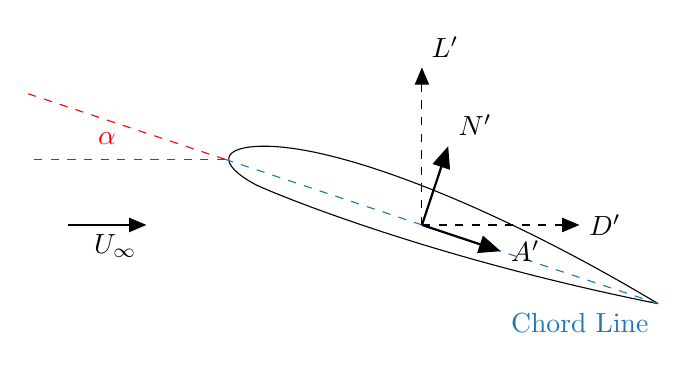
\begin{tikzpicture}
        \draw[rounded corners = 1cm] (6,-2)  .. controls (4, -0.8) and (2,0)  .. (0, 0) .. controls (1, -0.55) and (3, -1.4) .. (6,-2);
        \draw[dashed, blue] (0.5,-0.1666) -- (6,-2) node[anchor=north east] {Chord Line};
        \draw[dashed, red] (0.5,-0.1666) -- (-2,0.666);
        \draw[dashed, red] (0.5,-0.1666) -- (-2, -0.1666);
        \draw[red] (-1, 0.1) node {$\alpha$};
        \draw[->] (-1.5,-1) -- (-0.5,-1) node[anchor=north east] {$U_\infty$};
        \draw[thick,->] (3, -1) -- (3.3333, 0) node[anchor=south west] {$N'$};
        \draw[thick,->] (3, -1) -- (4, -1.333) node[anchor=west] {$A'$};
        \draw[dashed, ->] (3, -1) -- (3, 1) node[anchor=south west] {$L'$};
        \draw[dashed, ->] (3, -1) -- (5, -1) node[anchor=west] {$D'$};
    \end{tikzpicture}
    \caption{Definition of variables related to forces on an airfoil}
    \label{fig:airfoil_directions}
\end{figure}

Lift, drag, and moment are nondimensionalized using Equations \ref{eq:cl}, \ref{eq:cd}, and \ref{eq:cm} respectively where\\
$q_\infty\equiv\frac{1}{2}\rho_\infty U_\infty^2$ is the freestream dynamic pressure and $c$ is the chord length.

\begin{align}
    C_L &= \frac{L'}{q_\infty c}
    \label{eq:cl}\\
    C_D &= \frac{D'}{q_\infty c}
    \label{eq:cd}\\
    C_M &= \frac{M'}{q_\infty c^2}
    \label{eq:cm}
\end{align}

\subsection{Calculating Total Drag from Wake Velocity}
The drag force formulation from above ignores viscous effects, because this experiment cannot directly measure the shear force distribution over the surface of the airfoil. That means the force in Equation \ref{eq:drag} only gives pressure drag. Instead, total drag calculation is performed by performing a momentum balance in a control volume containing the airfoil, to determine how much the airfoil has decelerated the 
\begin{align}
    D' &= \rho\int_{\text{rake}} u (U_\infty - u) dy \label{eq:wake_drag}
\end{align}

\subsection{Stall}
Airfoil stall is characterized by a significant separation in flow from the airfoil surface resulting in several effects.\\
\\
When flow separation occurs, the $C_P$ distribution becomes flat in the region of separation.\\
\\
As $\alpha$ increases, $C_L$ increases linearly until it reaches a peak, and then falls sharply at stall.\\
\\
Flow separation incurs higher drag, resulting in higher $C_D$.\\
\\
$C_{M, LE}$ remains a nearly constant negative value until the airfoil stalls, at which point $C_{M, LE}$ becomes zero or slightly positive.\\
\\
Such conditions lead to unpredictable behaviour of an airfoil, and reduced aircraft controlability due to reduced effectiveness of aircraft control surfaces. It is important to understand the behaviour of a varying the angle of attack on the lift, drag, and moment characteristics of an airfoil to understand the limitations of the airfoil.



% -----------------------------------------------------------------------------
%   Experimental Set-Up
% -----------------------------------------------------------------------------


\section{Experimental Set-Up}

This details the lab setup and experimental procedure used in the experiment.

\subsection{Apparatus}

The Clark Y airfoil is 3D printed, with 19 small holes along the centerline of the span allowing pressure measurements over the surface. Pressure tap locations are presented in Table \ref{tab:pressure_taps}.

\begin{table}
    \centering
    \begin{tabular}{|c||c|c|c|c|c|c|c|c|c|c|}\hline
        x/c & 0 & 0.03 & 0.06 & 0.10 & 0.15 & 0.20 & 0.30 & 0.40 & 0.55 & 0.70 \\\hline
        Tap Number & 1 & 2 & 3 & 4 & 5 & 6 & 7 & 8 & 9 & 10\\\hline \hline
        x/c & 0.85 & 1.00 & 0.90 & 0.60 & 0.40 & 0.30 & 0.20 & 0.10 & 0.05&\\\hline
        Tap Number & 11 & 12 & 13 & 14 & 15 & 16 & 17 & 18 & 19&\\\hline
    \end{tabular}
    \caption{Static pressure tap locations for the test model. Taps 1 through 12 are on the top surface, while 13 thought 19 are on the bottom surface.}
    \label{tab:pressure_taps}
\end{table}

Tests are conducted in an ELD Model 402B subsonic open-return wind tunnel, with a 304.8 x 304.8 x 610 mm  square prismatic test section. The airfoil is shown installed in Figure \ref{fig:wind_tunnel_setup}. The airfoil is installed using a rotary mechanism to vary the angle of attack across runs, shown in Figure \ref{fig:aoa_select}.

\begin{figure}
    \centering
    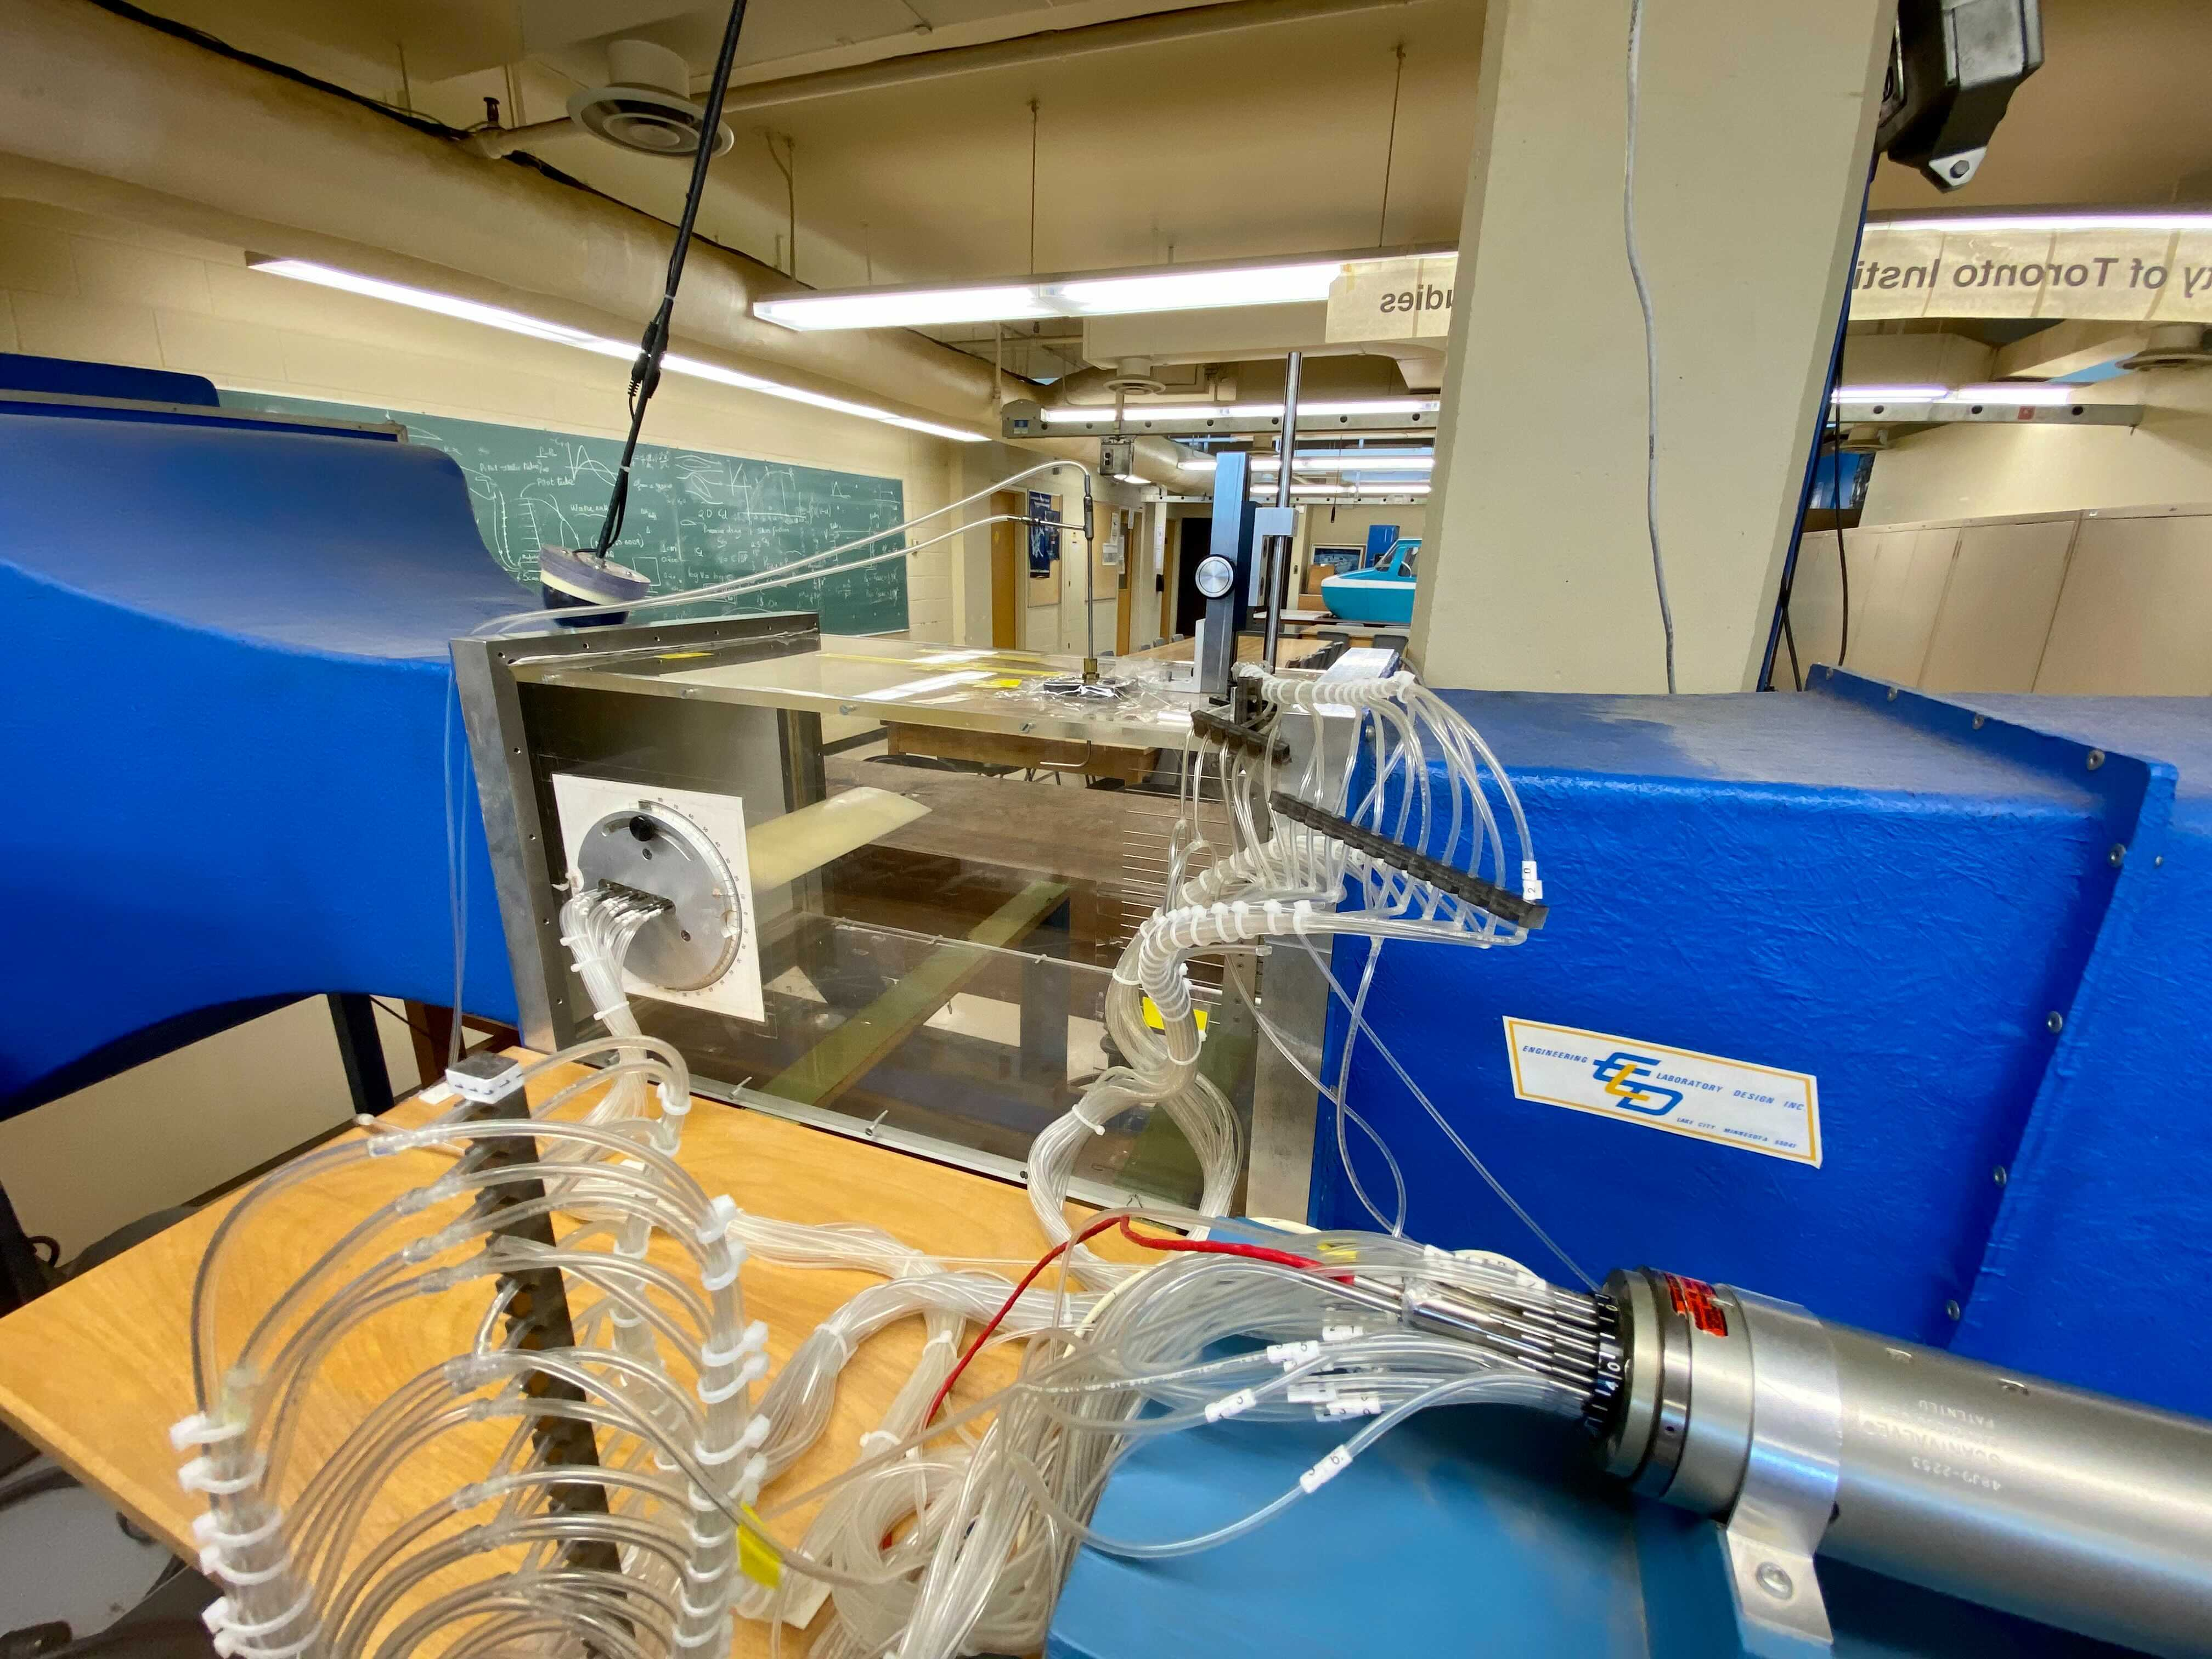
\includegraphics[width=0.6\textwidth]{Apparatus Pictures/wind_tunnel_setup.jpg}
    \caption{The wind tunnel section, with the 3D printed test model installed.}
    \label{fig:wind_tunnel_setup}
\end{figure}

\begin{figure}
    \centering
    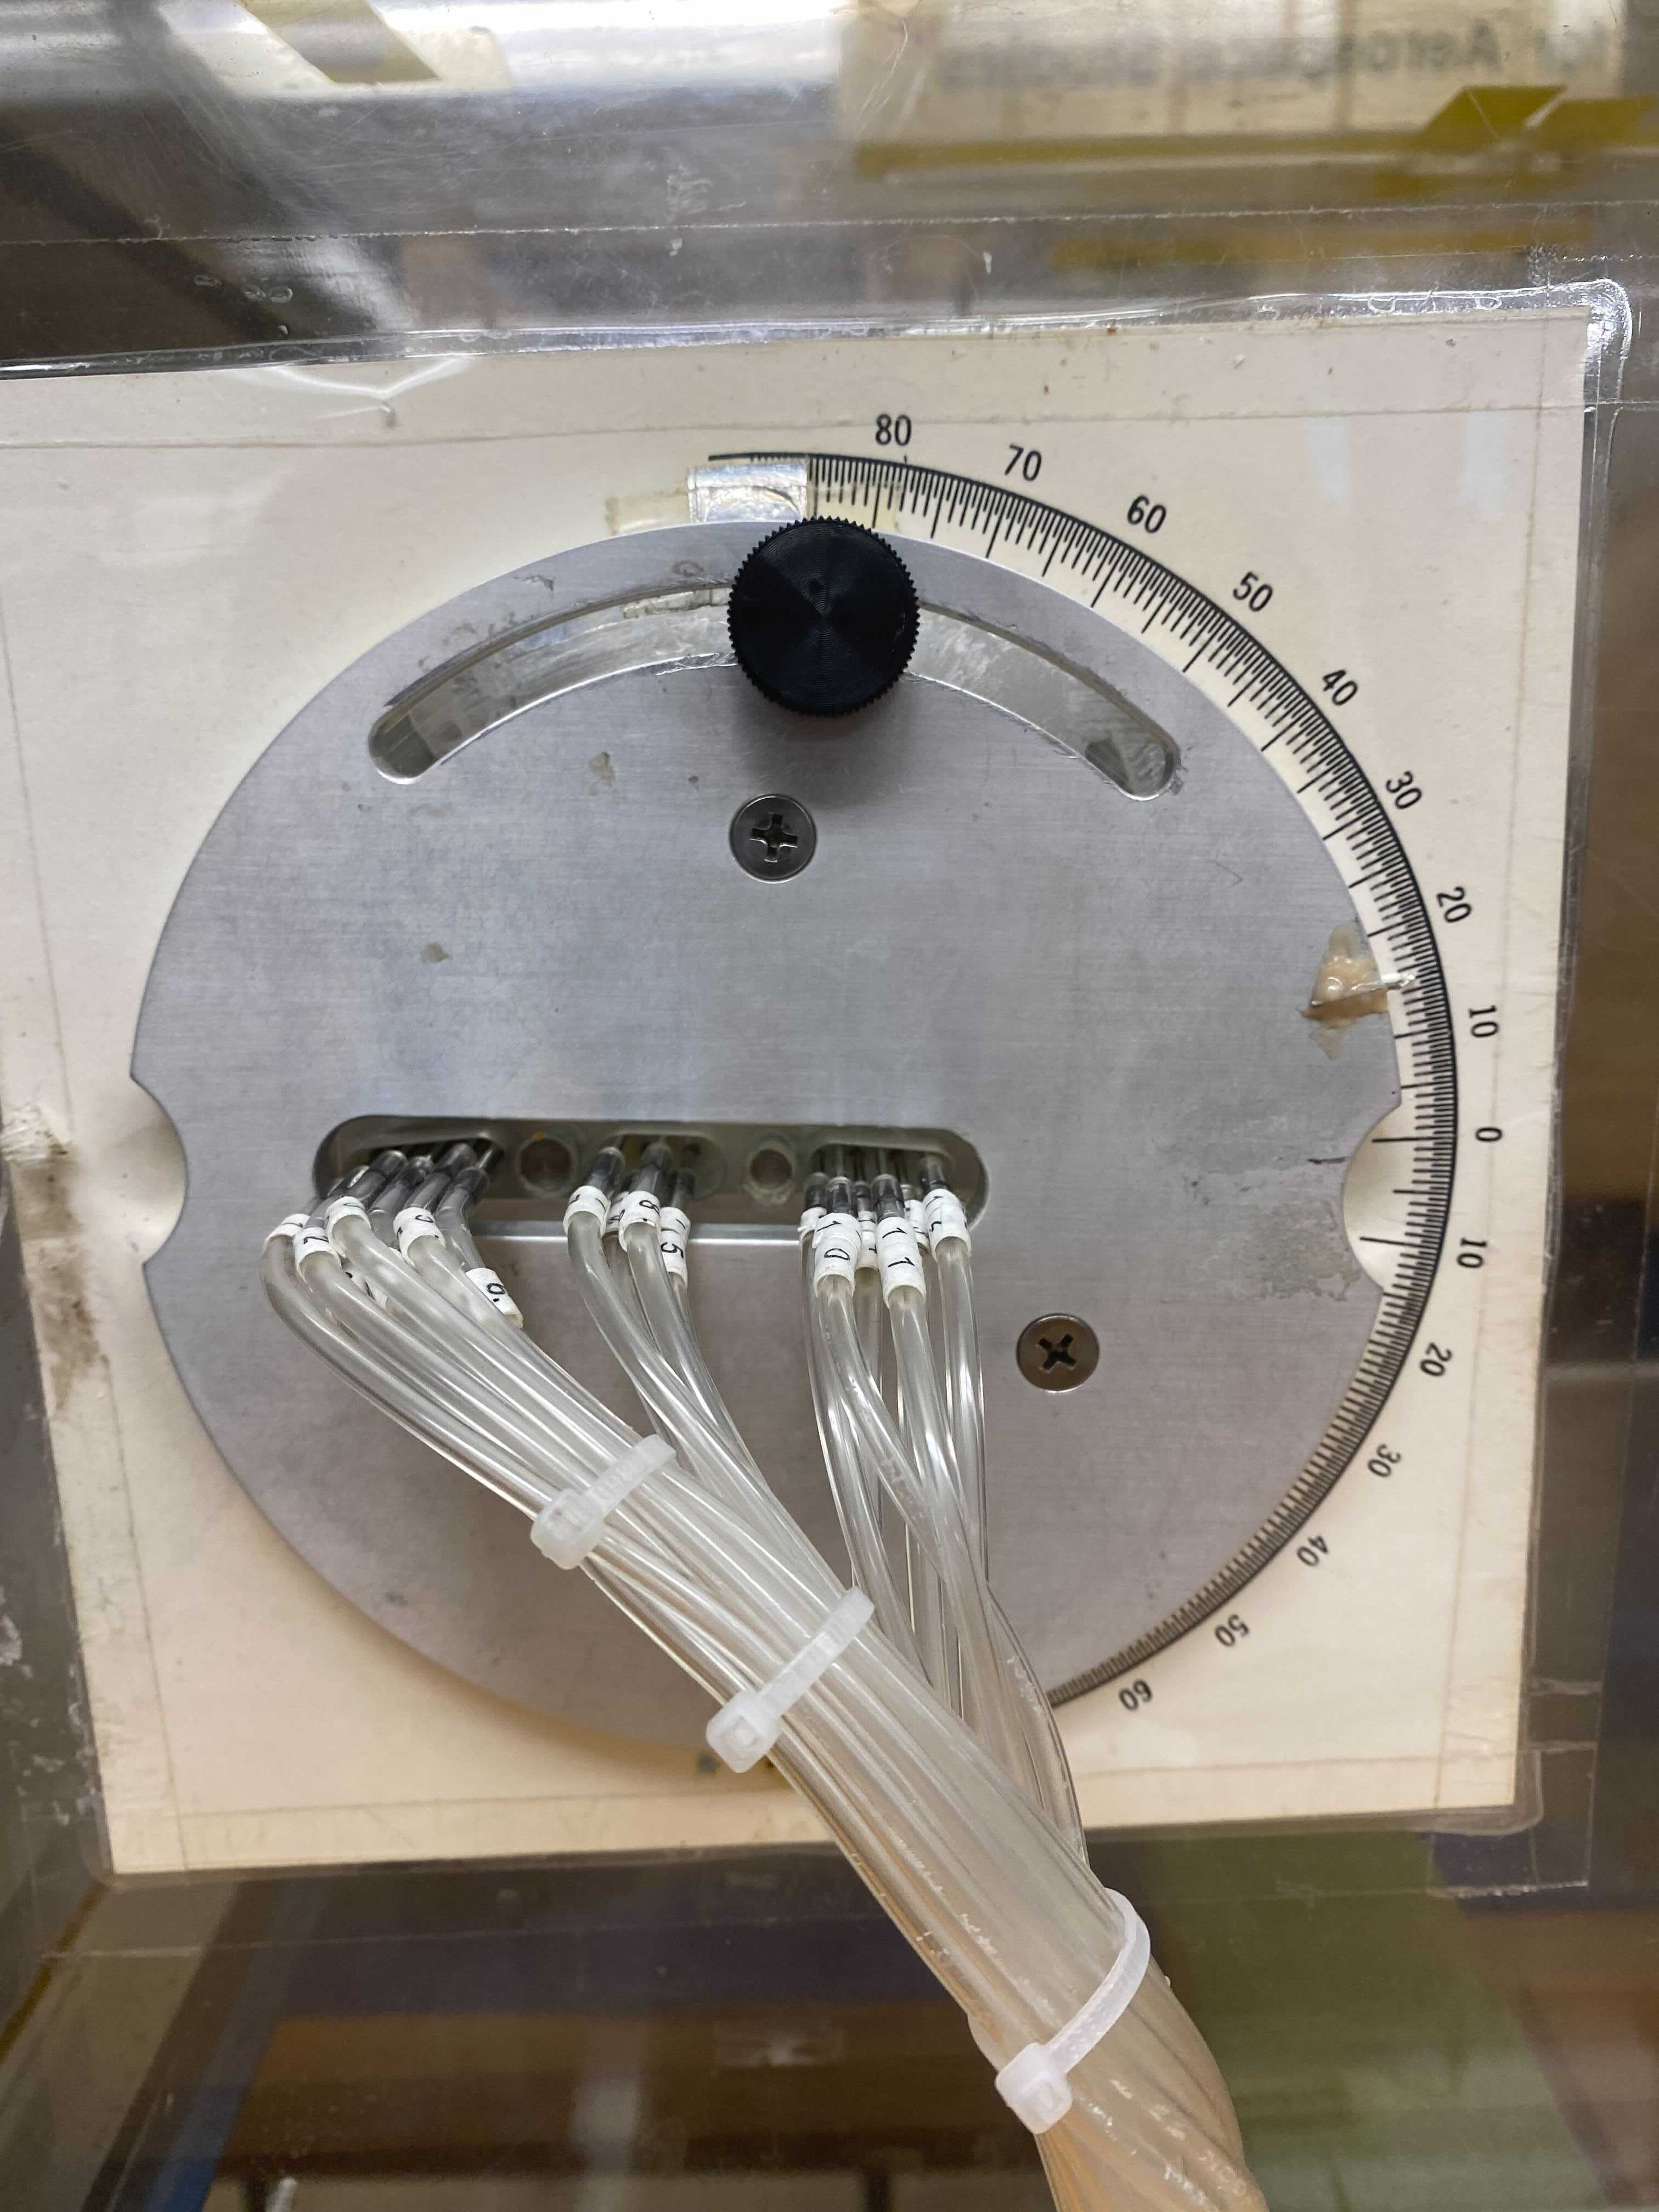
\includegraphics[width=0.4\textwidth]{Apparatus Pictures/aoa_selector.jpg}
    \caption{Adjustable rotary mechanism to hold the airfoil at different angles of attack.}
    \label{fig:aoa_select}
\end{figure}

In addition to 19 static pressure taps on the airfoil, there are 17 pitot tubes arranged as a rake, placed 27 cm downstream of the airfoil's trailing edge. A pitot-static tube placed upstream of the airfoil is used for wind tunnel speed measurement, with the pitot tube connected to a Betz manometer, and the static tube used as the reference pressure in the two measurement devices.

A total of 38 pressure tubes exit the wind tunnel; one is the upstream pitot tube connects to the Betz manometer, and the other 37 connect to the measurement devices. The latter 37 tubes are bifurcated to feed into a multi-channel Scanivalve-transducer system, and the other into an inclined manometer.

The Scanivalve system is pictured in Figure \ref{fig:scanivalve}. An analog pressure transducer is connected to the sampling and reference outputs of the Scanivalve. The connected sampling tube rapidly switches between 36 pressure tubes such that the pressure transducer measures the pressure difference between the sampled pressure and the reference pressure from the upstream static tube. The analog signal from the pressure transducer is fed into a data acquisition card, connected to a computer running MATLAB to collect data.

\begin{figure}[h]
    \centering
    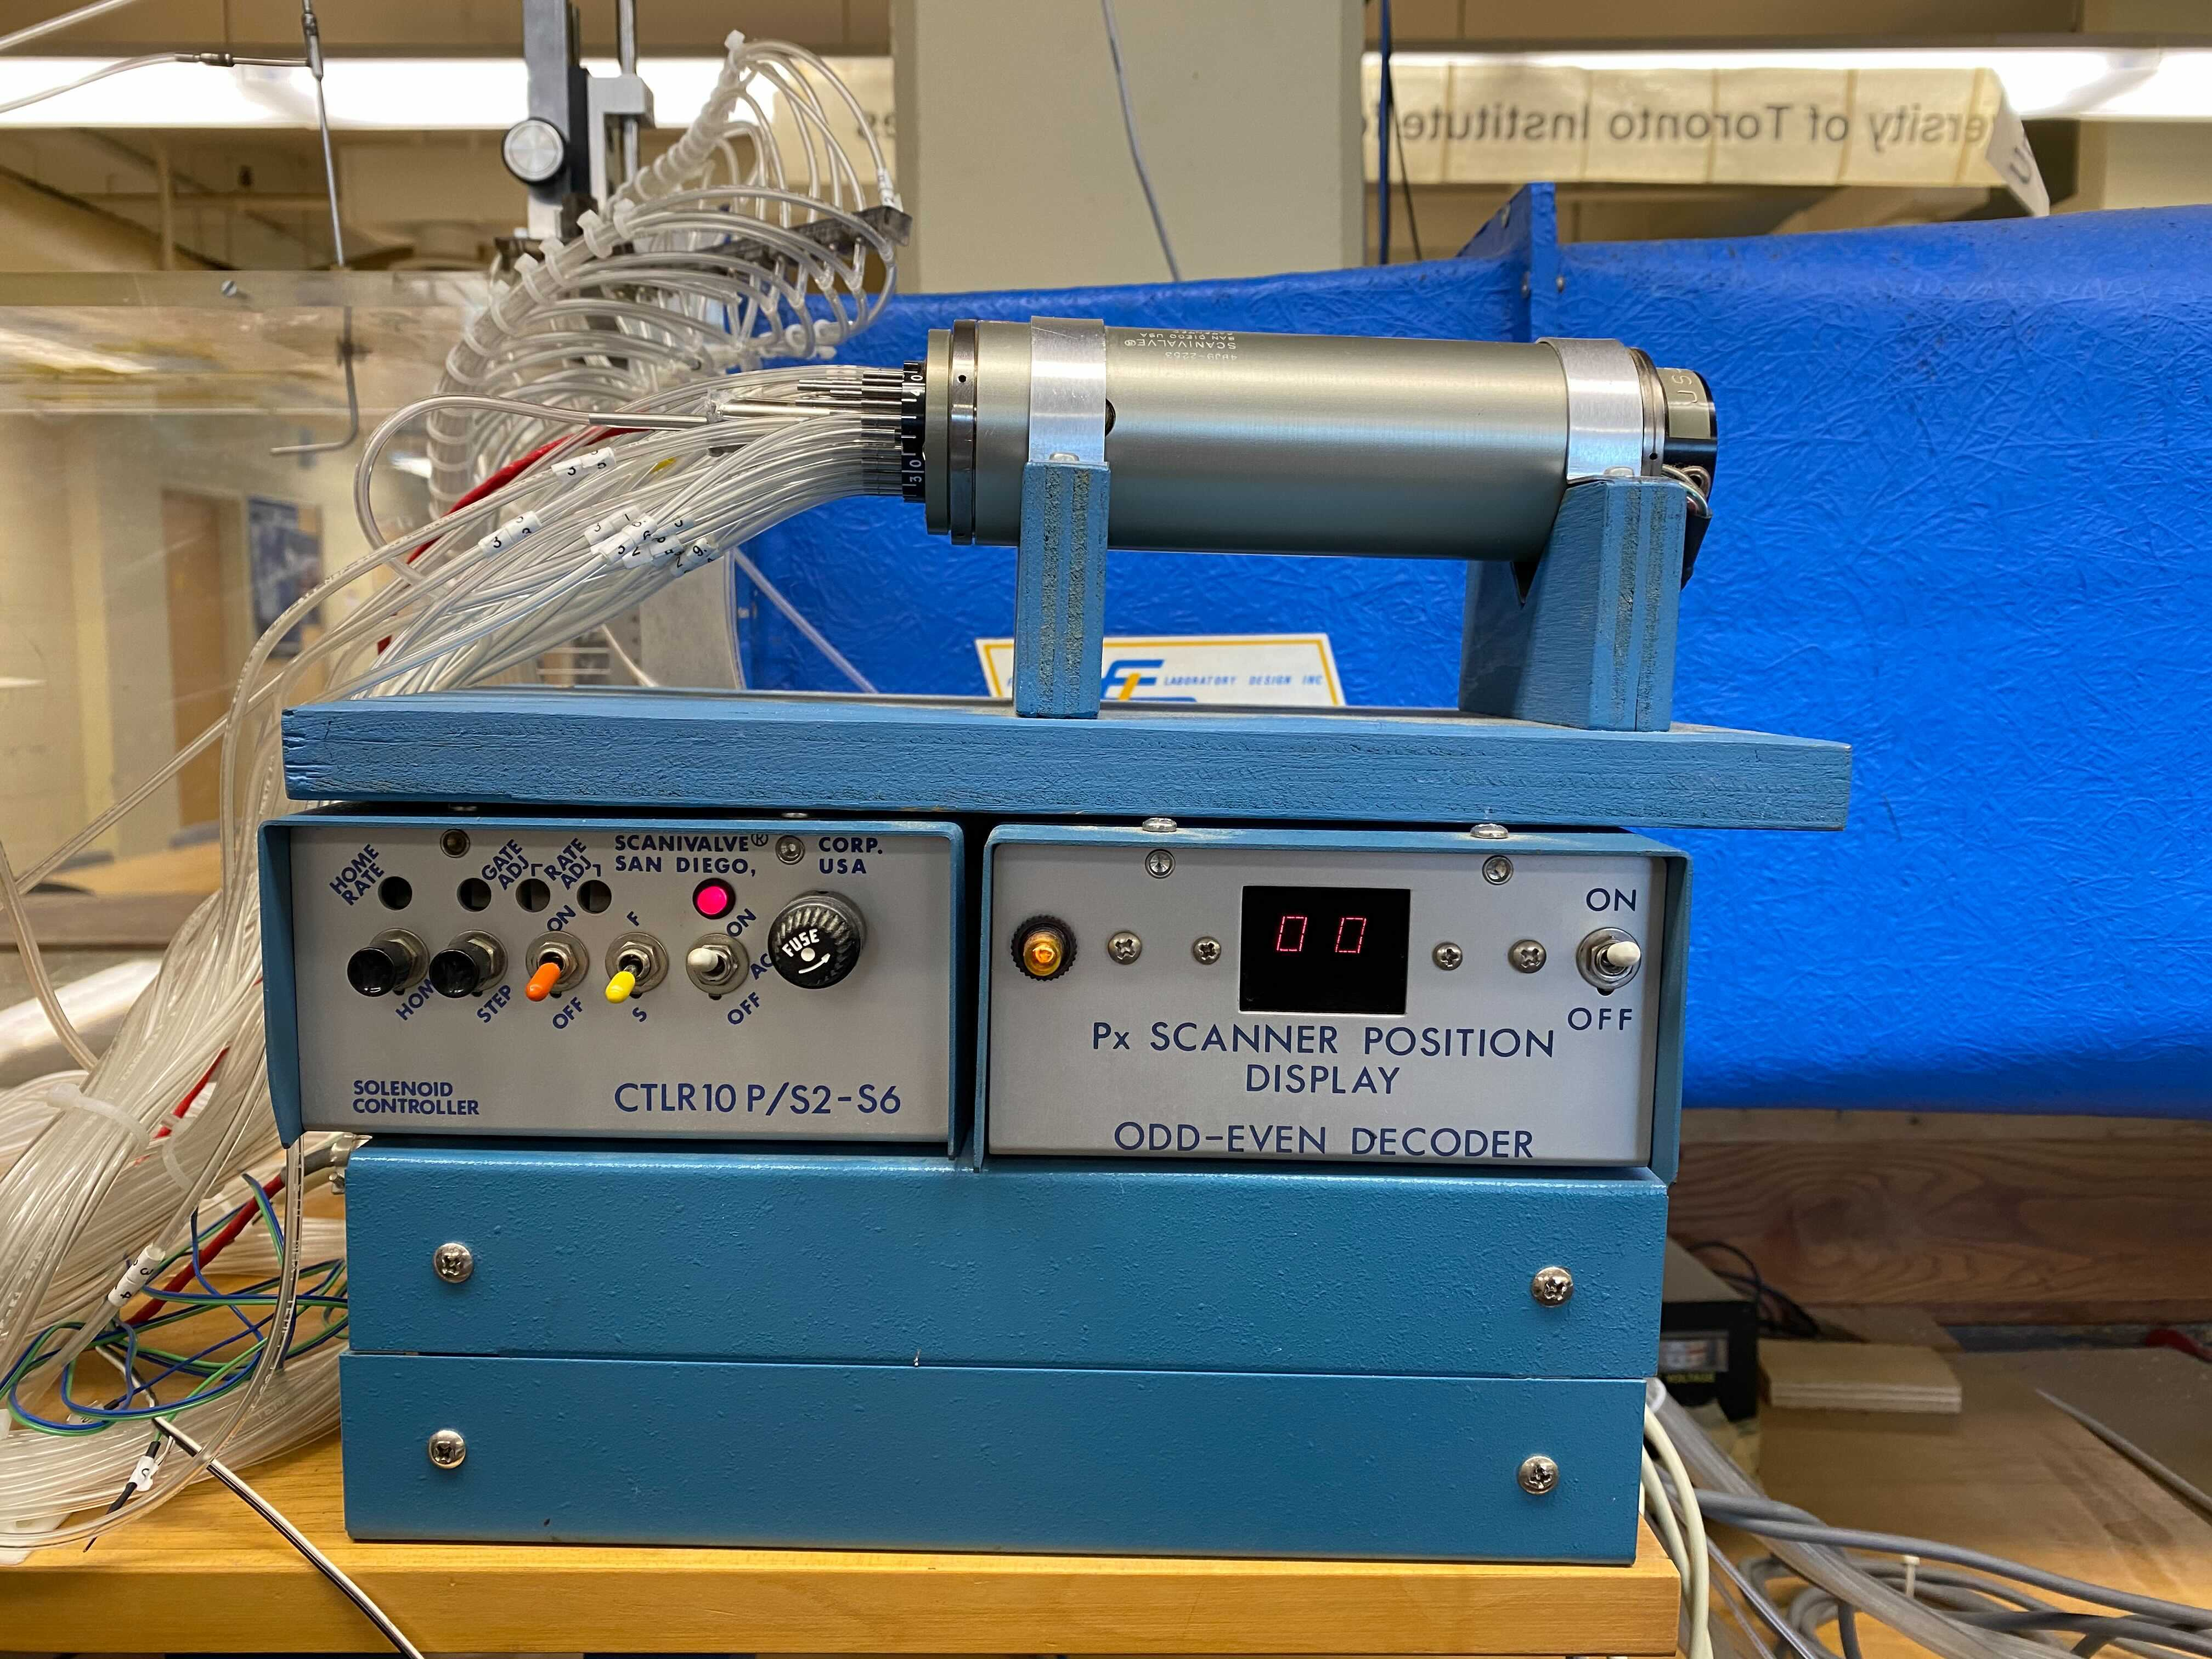
\includegraphics[width=0.4\textwidth]{Apparatus Pictures/scanivalve.jpg}
    \caption{Scanivalve system, connected to a pressure transcuder. The system allows rapid switching of each of the 36 channels to the transducer to sweep through all pressure measurements.}
    \label{fig:scanivalve}
\end{figure}

The inclined manometer takes in 36 input channels and one reference channel to measure the pressure difference between each of the 36 inputs compared to the reference. The reference pressure is set to that of the upstream static tube.

\begin{figure}[h]
    \centering
    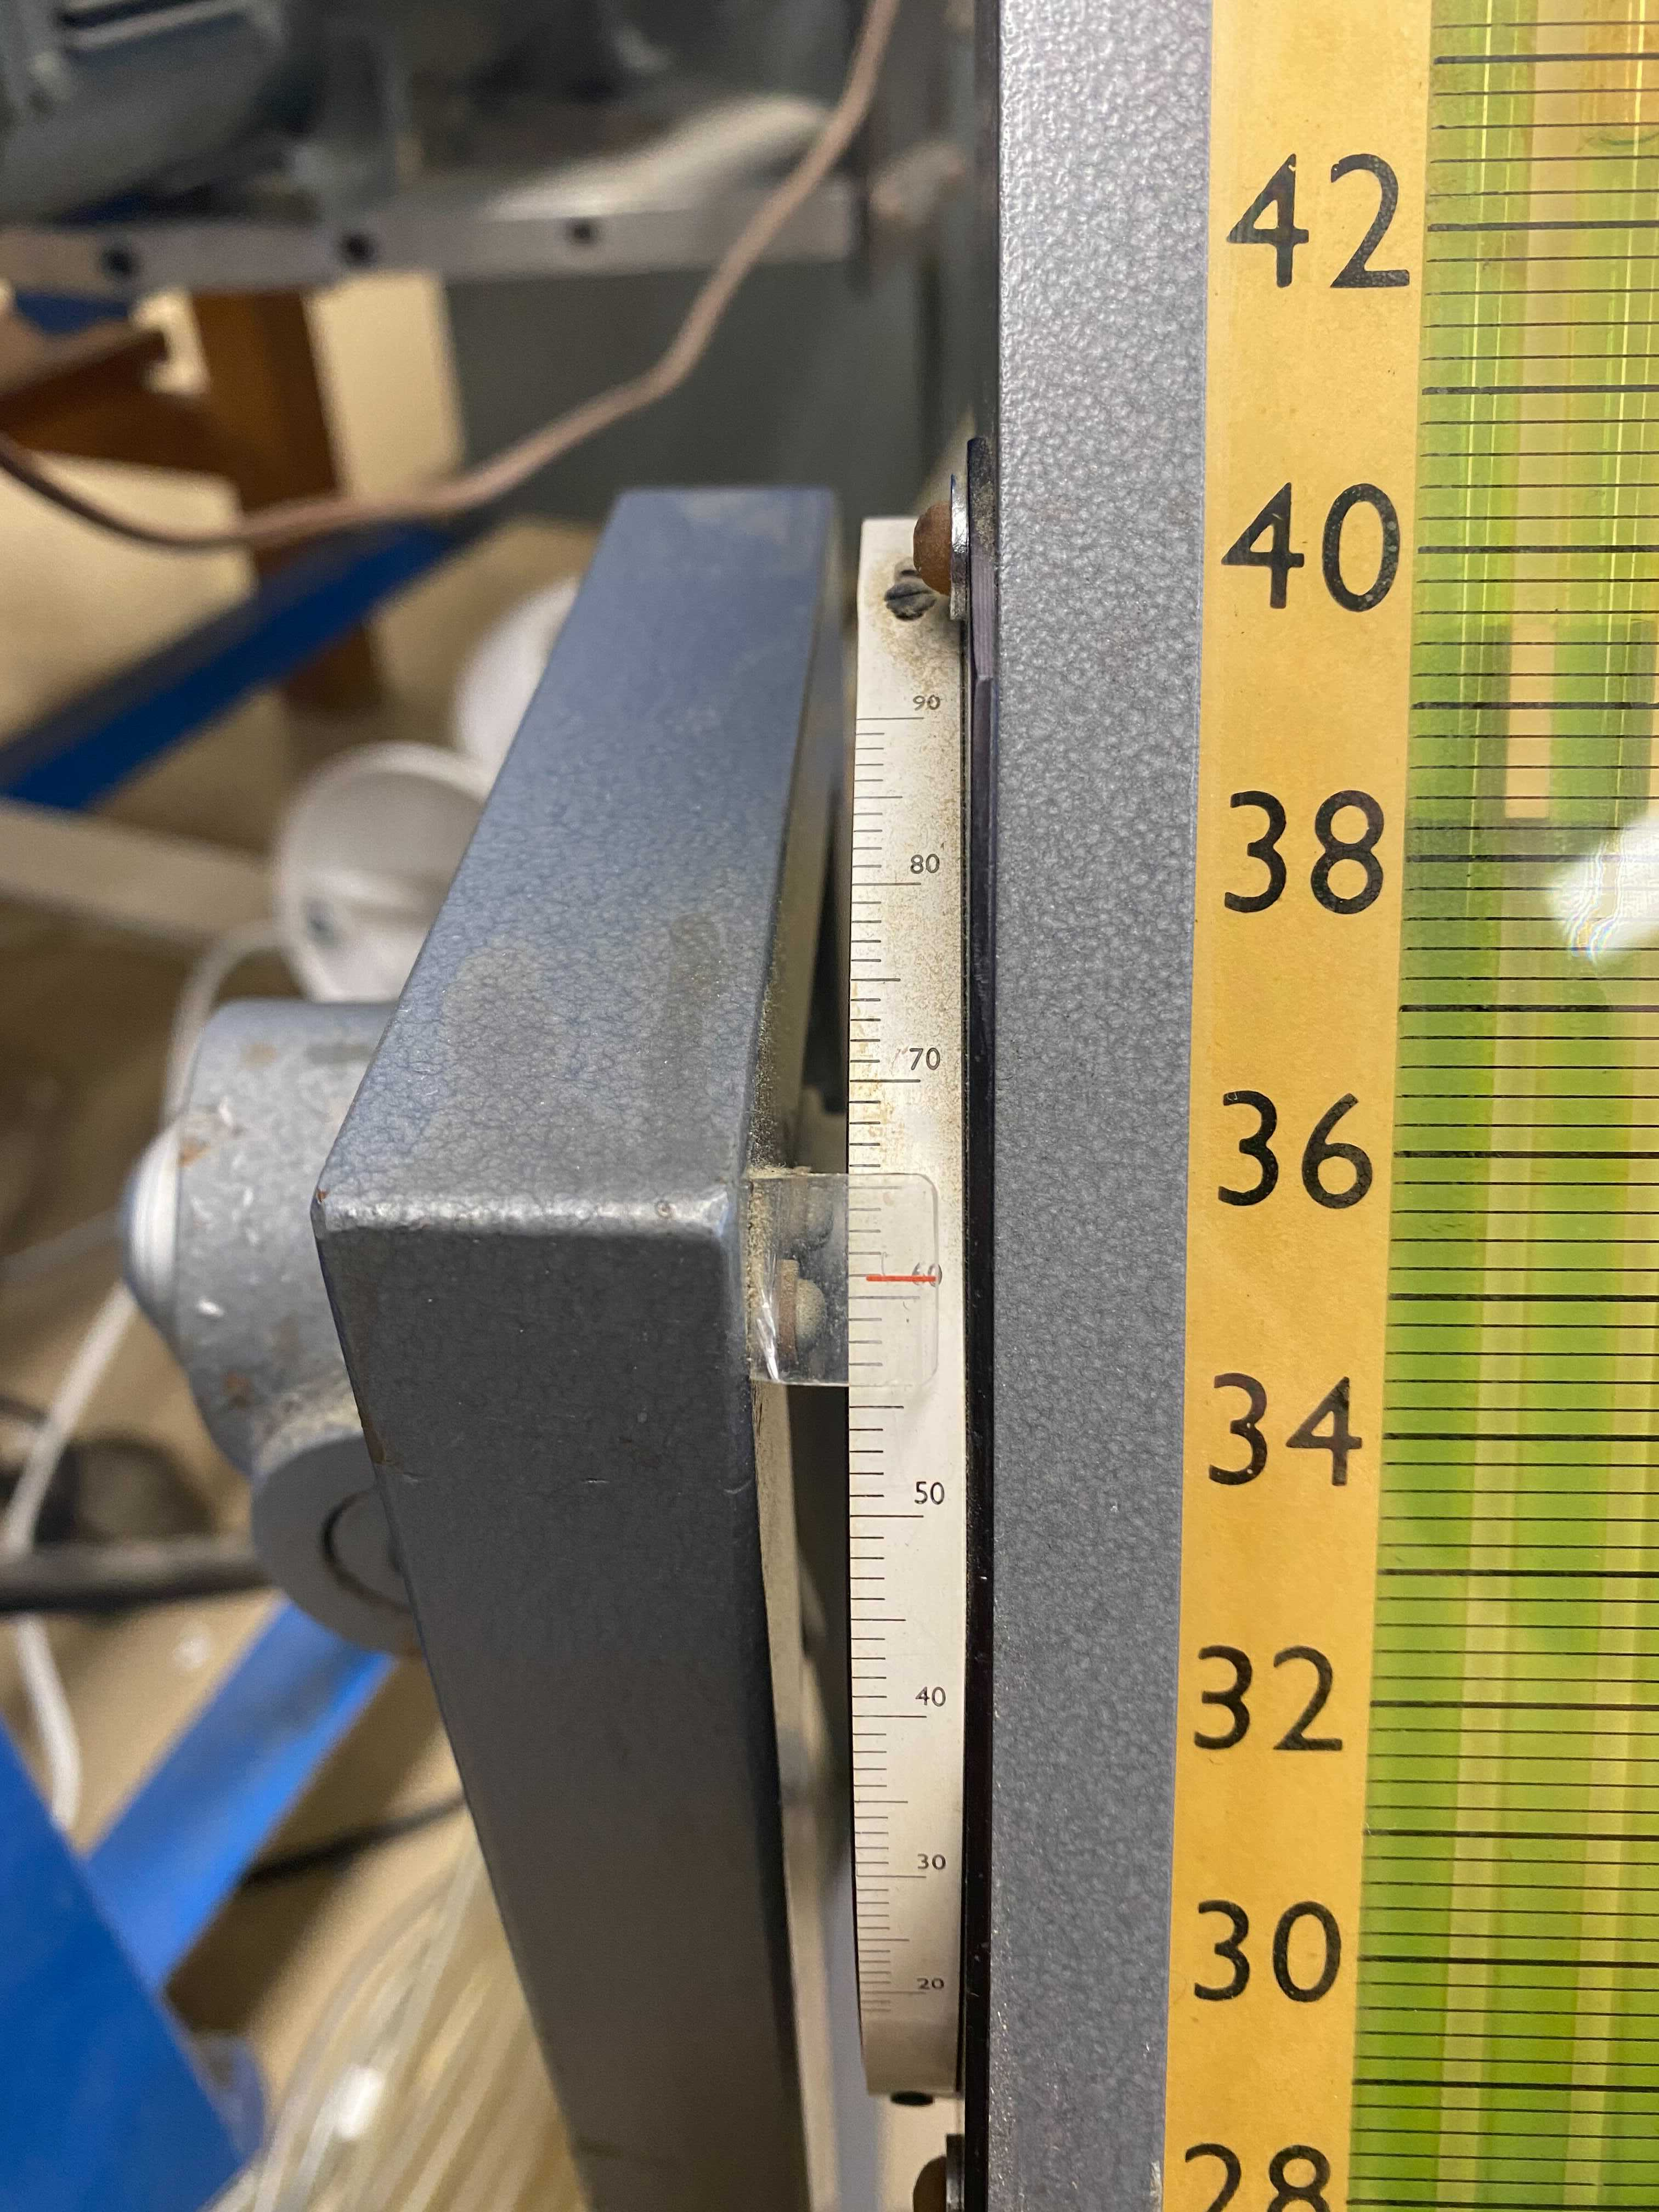
\includegraphics[width=0.4\textwidth]{Apparatus Pictures/inclined_manometer_slope_graduations.jpg}
    \caption{Inclined manometer.}
    \label{fig:manometer}
\end{figure}

\subsection{Procedure}

% What is measured and how it is acquired.

The procedure used for acquisition of pressure measurements is as follows:

\begin{enumerate}

    \item The sample frequency and data acquisition time are determined such that the pressure transducer measurements admit a $\pm 1\%$ accuracy. The wind tunnel is set to a speed of $110\si{km.h^{-1}}$. A series of representative measurements from the pressure transducer output are taken and autocorrelated to determine the sample frequency and data acquisition time required for $\pm 1\%$ accuracy.
    
    \item The calibration curve for the pressure transducer is constructed next. This allows interpolated conversion from voltage-pressure representations of pressure transducer into equivalent pressure values. The curve is constructed by taking ten different voltage-pressure measurements are taken at varying wind tunnel speeds using scanivalve readings while finding the corresponding pressure measurements using the Betz manometer. This correspondence between representations is used to calibrate the pressure-voltage curve of the transducer.
    
    \item The wind tunnel speed is set back to $110\si{km.h^{-1}}$ and wind tunnel's pitot-static pressure difference is measured to calculate the actual wind speed experiences in the wind tunnel.
    
    \item Next, the angle of attack is changed in the positive and negative directions to determine the stall angle values. Using this information, it is determined what angles of attack would be useful to measure to accurately represent the airfoil properties up to and past stall conditions. The angle of attack values chosen were \numlist{0;3;6;8;10;11;13;15;16;17;20} degrees.

    \item Cycling through each angle of attack, the pressure distribution is measured along the top and bottom surfaces of the airfoil in addition to the pressure distribution in the airfoils wake. These values are measured by reading the fluid height changes from the inclined manometer. To get greater precision in the wake measurements, the wake rake is displaced by $5\si{mm}$ for a second round of measurements to fill the gaps between each rake tube. Pressure measurements are taken using two methods: (1) the pressure transducer fed by the scanivalve device and (2) the inclined manometer.

\end{enumerate}

Once the pressure measurements were taken, the data is pre-processed to obtain pressure distributions over the airfoil and in its wake. This pre-processing follows the following procedure depending on the measurement method.

\begin{enumerate}

    \item For data calculated using the pressure transducer, the calibration curve for the pressure transducer is used to convert raw data into equivalent pressure readings, using an interpolation script.

    \item For the inclined manometer approach, the data is captured in images which we annotate using a web based data extraction tool for converting our image embedded data to csv files.\cite{Rohatgi2020} In this annotation stage, we specify graph boundaries and the scale of the graph. We then select the peaks of each manometer tube. The program will then interpolate between the boundaries to get a measure of our selection. Distortions in the image can cause nonlinear length scales that can provide error into the data acquisition as discussed in section \ref{sec:non_quantifiable_sources_of_error}. From the csv data, the change in static pressure is determined from the change of fluid height for each manometer tube compared to an "at-rest" state which and using Bernoulli's relation.

\end{enumerate}

After the data is pre-processed, the data is analyzed to determine the lift, moment, and drag coefficients as well as a measure of the lift, moment, and pressure drag of the airfoil up to and past the point of stall. The analysis is done using the methods described in section \ref{sec:introduction_and_background}.

%% TODO: mention image analysis process

% -----------------------------------------------------------------------------
%   Results and Discussion
% -----------------------------------------------------------------------------


\section{Results and Discussion}

\subsection{XFOIL Reference}
Results in this section are compared to data obtained from \textit{XFOIL}, a free airfoil analysis software. Reference results with XFOIL are obtained from analysis of the .dat file obtained from \href{http://airfoiltools.com/airfoil/details?airfoil=clarky-il}{airfoiltools.com}, using 240 panels nodes in the viscous solver mode at $Re = 200000$. Pressure distributions, and the dimensionless coefficients are determined for all $\alpha$ values used in the experiment.

\subsection{Wake Velocity Profile}
Wake velocities are obtained from total pressure measurements in the wake to determine the flow velocity distribution over the height of the pressure rake. The freestream velocity $U_\infty$ is taken to be the mean between the measured velocity at the uppermost and bottommost rakes. Resulting total drag is computed numericall using Equation \ref{fig:total_drag} and \verb|trapz| in MATLAB. The drag coefficient $C_D$ is obtained using Equation \ref{eq:cd}. Wake velocity and 
\begin{figure}
    \centering
    \begin{subfigure}[b]{0.45\textwidth}
         \centering
         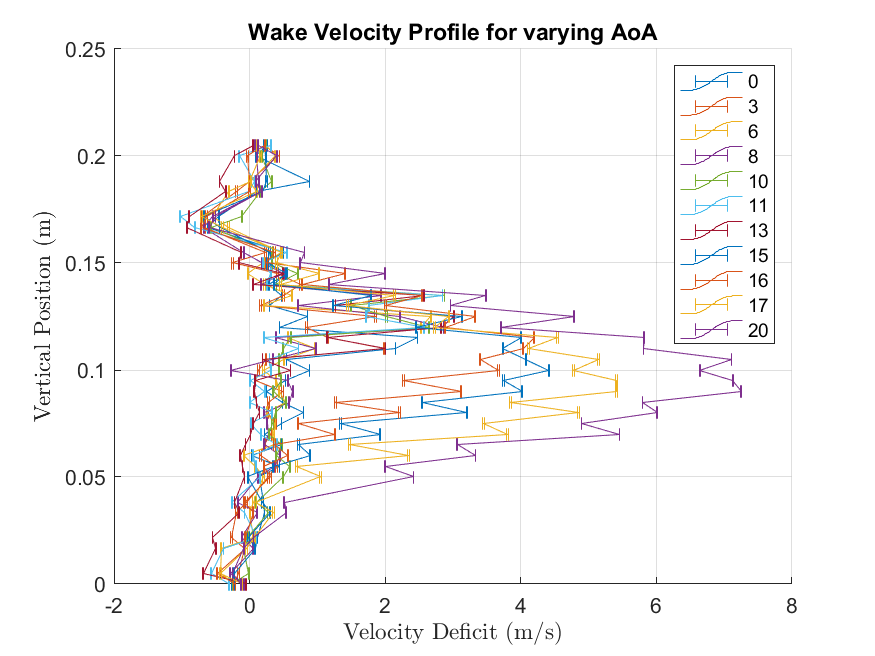
\includegraphics[width=\textwidth]{figures/scanivalve_wake_velocities.png}
         \caption{}
         \label{fig:scanivalve_wake_velocity}
     \end{subfigure}
     \begin{subfigure}[b]{0.45\textwidth}
         \centering
         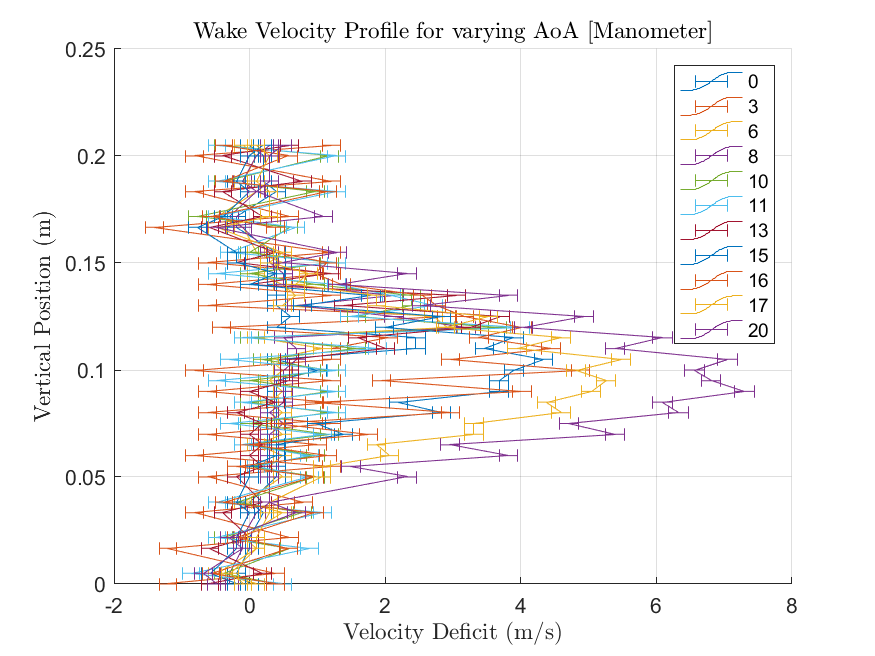
\includegraphics[width=\textwidth]{figures/manometer_wake_velocities.png}
         \caption{}
         \label{fig:manometer_wake_velocity}
     \end{subfigure}
    \caption{Velocity deficit $U_\infty - u$ in the wake for each $\alpha$, from both the scanivalve and manometer data.}
    \label{fig:wake_velocities}
\end{figure}
\begin{figure}
    \centering
    \begin{subfigure}[b]{0.45\textwidth}
         \centering
         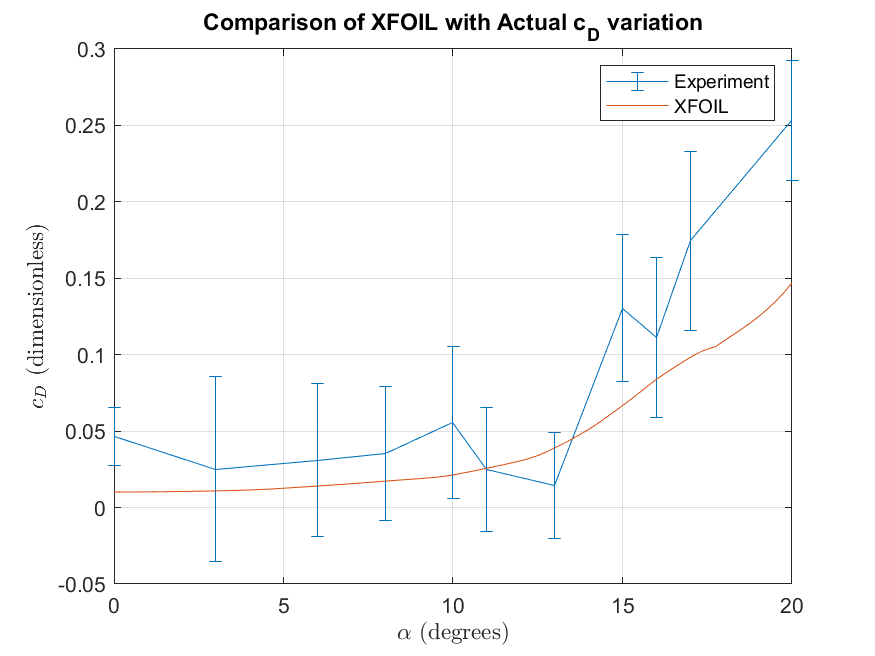
\includegraphics[width=\textwidth]{figures/scanivalve_cd.png}
         \caption{}
         \label{fig:scanivalve_wake_velocity}
     \end{subfigure}
     \begin{subfigure}[b]{0.45\textwidth}
         \centering
         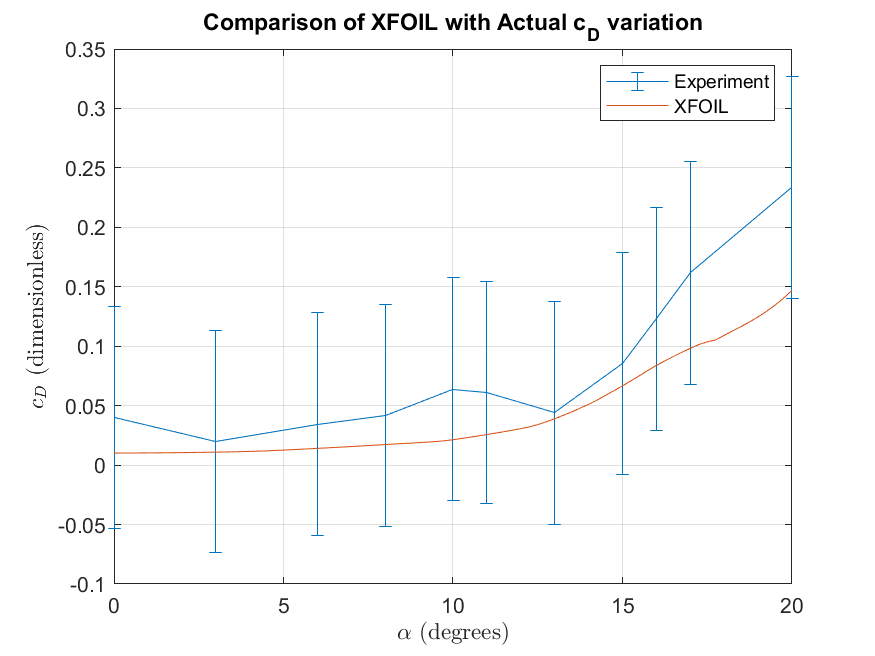
\includegraphics[width=\textwidth]{figures/manometer_cd.png}
         \caption{}
         \label{fig:manometer_wake_velocity}
     \end{subfigure}
    \caption{Total drag coefficient versus XFOIL.}
    \label{fig:total_drag_coefficient}
\end{figure}

\subsection{Coefficient of Lift, Pressure Drag, and Moment}

\subsection{Pressure Drag and Total Drag Comparison}
\begin{table}[h]
\centering
\begin{tabular}{p{3cm}p{3cm}p{3cm}p{3cm}p{3cm}}
\toprule
$\alpha^\circ$ & $D'_p$ (Scanivalve) & $D'_p$ (Manometer) & $D'$ (Scanivalve) & $D'$ (Manometer) \\
\midrule
 $0.00\pm0.25$ \\
 $3.00\pm0.25$ \\
 $6.00\pm0.25$ \\
 $8.00\pm0.25$ \\
$10.00\pm0.25$ \\
$11.00\pm0.25$ \\
$13.00\pm0.25$ \\
$15.00\pm0.25$ \\
$16.00\pm0.25$ \\
$17.00\pm0.25$ \\
$20.00\pm0.25$ \\
\bottomrule
\end{tabular}
\caption{Comparison of pressure and total drag force per unit span.}
\label{tab:pressure_comparison}
\end{table}
\begin{figure}
    \centering
    \begin{subfigure}[b]{0.45\textwidth}
         \centering
         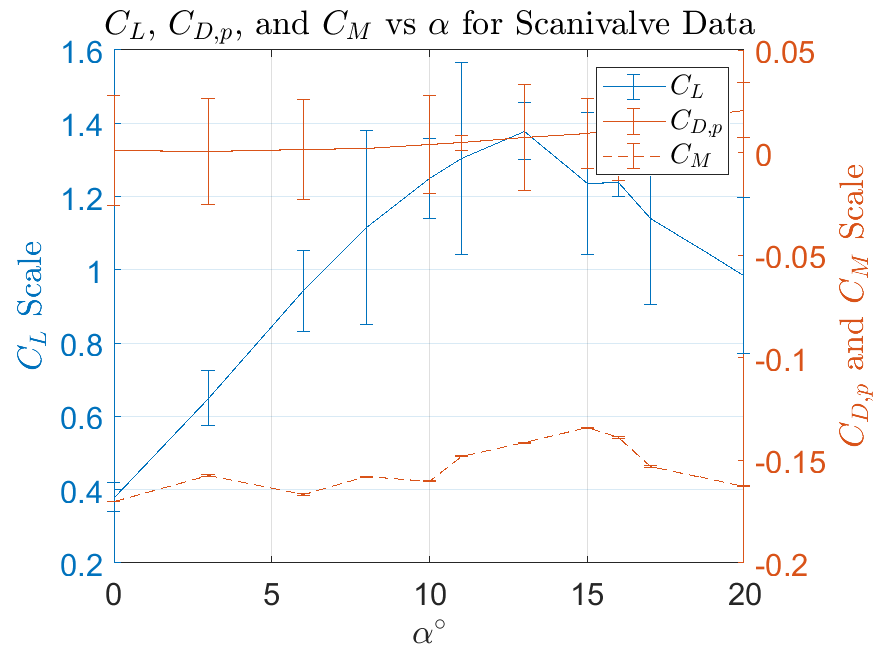
\includegraphics[width=\textwidth]{figures/scanivalve_cl_cd_cm.png}
         \caption{Coefficients calculated from scanivalve data.}
         \label{fig:scani_coeff}
     \end{subfigure}
     \begin{subfigure}[b]{0.45\textwidth}
         \centering
         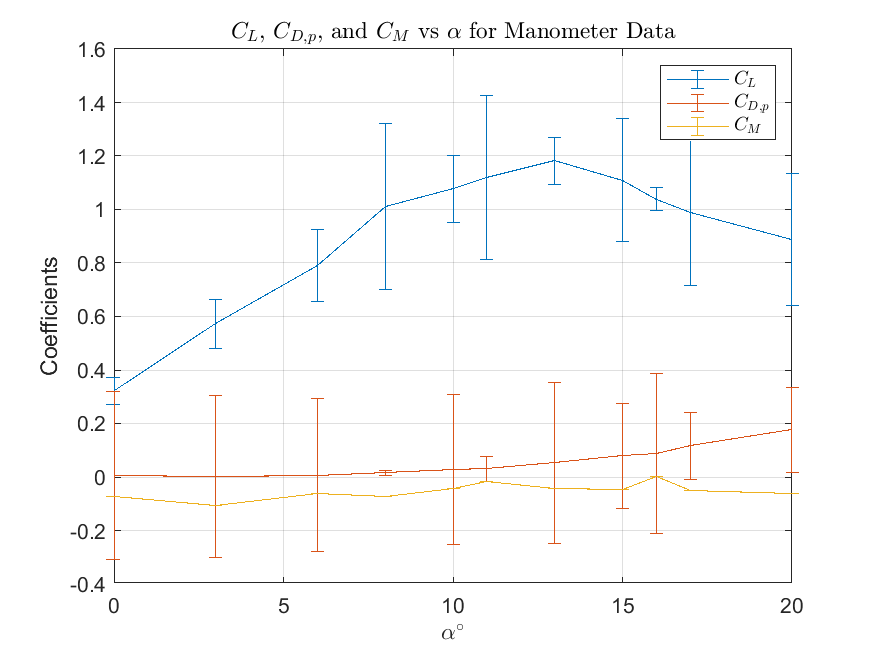
\includegraphics[width=\textwidth]{figures/manometer_cl_cd_cm.png}
         \caption{Coefficients calculated from manometer data.}
         \label{fig:mano_coeff}
     \end{subfigure}
    \caption{Empirically determined coefficients of lift, pressure drag, and moment.}
    \label{fig:coeffs}
\end{figure}

\begin{figure}
    \centering
    \begin{subfigure}[b]{0.45\textwidth}
         \centering
         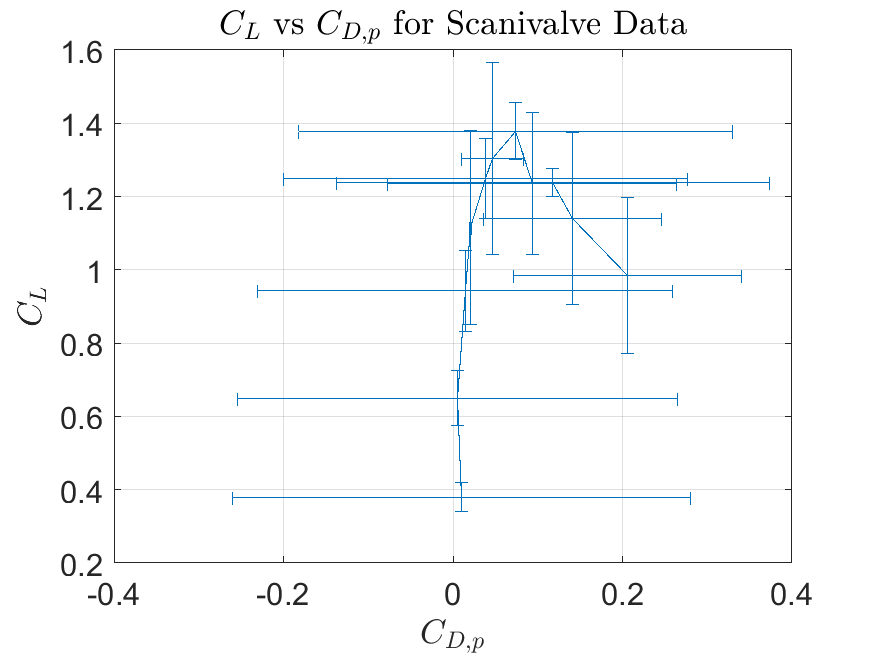
\includegraphics[width=\textwidth]{figures/scanivalve_cl_vs_cd.png}
         \caption{$C_L$ vs $C_{D,p}$ from scanivalve data.}
         \label{fig:scani_cL_cD}
     \end{subfigure}
     \begin{subfigure}[b]{0.45\textwidth}
         \centering
         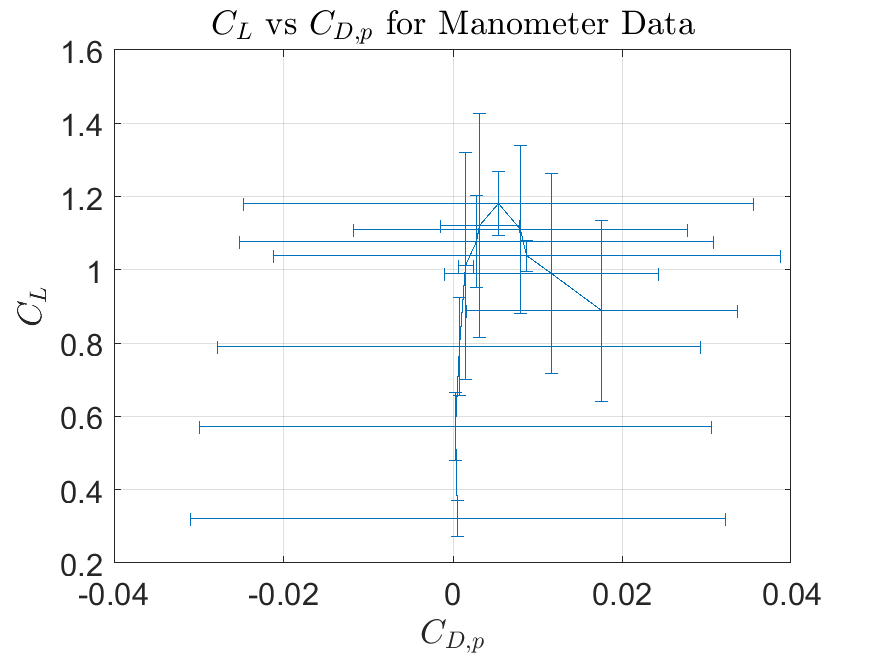
\includegraphics[width=\textwidth]{figures/manometer_cl_vs_cd.png}
         \caption{$C_L$ vs $C_{D,p}$ from manometer data.}
         \label{fig:mano_cL_cD}
     \end{subfigure}
    \caption{Empirically determined $C_L$ vs $C_{D,p}$ curves.}
    \label{fig:cL_vs_cD}
\end{figure}

\begin{table}[h]
\centering
\begin{tabular}{p{3cm}p{3cm}p{3cm}p{3cm}}
\toprule
$\alpha^\circ$ & $C_L$ & $C_{D,p}$ & $C_M$ \\
\midrule
 $0.00\pm0.25$ & $0.380\pm0.039$ & $0.0100236\pm0.27$ &  $-0.170094\pm0.000050$ \\
 $3.00\pm0.25$ & $0.650\pm0.076$ & $0.01\pm0.26$ & $-0.15733\pm0.00051$ \\
 $6.00\pm0.25$ & $0.94\pm0.11$ & $0.01\pm0.24$ &  $-0.16652\pm0.00035$ \\
 $8.00\pm0.25$ & $1.12\pm0.26$ &  $0.02068\pm0.00082$ & $-0.15797\pm0.00026$ \\
$10.00\pm0.25$ & $1.25\pm0.11$ & $0.04\pm0.24$ & $-0.16007\pm0.00033$ \\
$11.00\pm0.25$ & $1.30\pm0.26$ & $0.05\pm0.037$ &  $-0.14797\pm0.00022$ \\
$13.00\pm0.25$ & $1.379\pm0.077$ &  $0.07\pm0.26$ & $-0.14144\pm0.00016$ \\
$15.00\pm0.25$ & $1.24\pm0.19$ & $0.09\pm0.17$ & $-0.13417\pm0.00032$ \\
$16.00\pm0.25$ & $1.238\pm0.038$ & $0.12\pm0.26$ & $-0.13876\pm0.00037$ \\
$17.00\pm0.25$ &  $1.14\pm0.23$ & $0.14\pm0.11$ &  $-0.15305\pm0.00048$ \\
$20.00\pm0.25$ & $0.99\pm0.21$ &  $0.21\pm0.13$ & $-0.16259\pm0.00021$ \\
\bottomrule
\end{tabular}
\caption{Coefficients of lift, pressure drag, and moment for the scanivalve data.}
\label{tab:scani_coeff}
\end{table}

\begin{table}[h]
\centering
\begin{tabular}{p{3cm}p{3cm}p{3cm}p{3cm}}
\toprule
$\alpha^\circ$ & $C_L$ & $C_{D,p}$ & $C_M$ \\
\midrule
 $0.00\pm0.25$ & $0.322\pm0.050$ & $0.01\pm0.32$ &  $-0.072506\pm0.000050$ \\
 $3.00\pm0.25$ & $0.573\pm0.092$ &   $0.00\pm0.30$ & $-0.10605\pm0.00051$ \\
 $6.00\pm0.25$ & $0.79\pm0.13$ &  $0.0074\pm0.28$ &  $-0.06257\pm0.00035$ \\
 $8.00\pm0.25$ & $1.01\pm0.31$ & $0.0153\pm0.0086$ & $-0.071424\pm0.00026$ \\
$10.00\pm0.25$ & $1.08\pm0.13$ & $0.03\pm0.28$ & $-0.04364\pm0.00033$ \\
$11.00\pm0.25$ & $1.12\pm0.31$ & $0.032\pm0.047$ & $-0.01843\pm0.00022$ \\
$13.00\pm0.25$ & $1.181\pm0.087$ &  $0.05\pm0.30$ & $-0.04153\pm0.00016$ \\
$15.00\pm0.25$ & $1.11\pm0.23$ & $0.08\pm0.20$ & $-0.04825\pm0.00032$ \\
$16.00\pm0.25$ & $1.038\pm0.042$ & $0.09\pm0.30$ &  $0.00178\pm0.00037$ \\
$17.00\pm0.25$ & $0.99\pm0.27$ & $0.12\pm0.13$ &  $-0.05075\pm0.00048$ \\
$20.00\pm0.25$ & $0.89\pm0.25$ & $0.18\pm0.16$ & $-0.06027\pm0.00021$ \\
\bottomrule
\end{tabular}
\caption{Coefficients of lift, pressure drag, and moment for the manometer data.}
\label{tab:mano_coeff}
\end{table}

\subsection{Comparison with other experiments}

Experimental performance data of a Clark Y airfoil is available in literature
\cite{lyon_broeren_giguere_gopalarathnam_selig_1997}.


% -----------------------------------------------------------------------------
%   Sources of Error
% -----------------------------------------------------------------------------


\section{Sources of Error}

\subsection{Quantifiable Sources of Errors}
\begin{table}[H]
\begin{center}
    \begin{tabular}{ll}
        \toprule
        \multicolumn{2}{c}{Quantifiable Error}\\
        \midrule
        Manometer Uncertainty Reading & $\pm 1 mm$\\
        Manometer Angle Uncertainty & $\pm 0.5^\circ$ \\
        Scanivalve Precision & Acquired from autocorrelation using port 36 in each trial. See table (x)\\
        Scanivalve Bias & Assume to be 0 \\
        Calibration Coefficients & Assume to be 0\\
        \bottomrule
\end{tabular}
\end{center}
\caption{Quantifiable Sources of Error, Tabulated}
\label{tab:quant_error}
\end{table}

\subsection{Non-Quantifiable Sources of Error}
\label{sec:non_quantifiable_sources_of_error}

The experimental setup contained various areas of non-quantifiable sources of error such as the low frequency response in the pressure tubes, the precision error of the manometer, the turbulence in the airfoil wake, and the distortion effect in image acquisition.\newline

\noindent
For the pressure experienced in the wind tunnel to be measured by the scanivalve or manometer, the pressure changes had to travel down a series of long tubes before reaching the measuring devices. This long transit will cause a damping in the strength of pressure gradients and thus the extent or pressure changes at the manometer and scanivalve ends. This effect will result in a low frequency response of our measurements.\newline

\noindent
Two other sources of error arise from the unpredictable fluctuations in pressure information. Specifically, the imaging method of data acquisition from the manometer took a snapshot of the measurements in time. Not gaining a time series of the data prevents us from knowing the precision error of our measurements which would allow us to quantify the probability of getting the measurements we received from the distribution from all possible fluctuations. Another aspect of pressure fluctuations was seen in the airfoil's wake whose turbulent flow created random undulations in the measured pressure. The snapshot of this unsteady flow as measured by the rake device failed to capture the time series of these fluctuations, again, preventing the quantification of such oscillations in the airfoil wake velocity.\newline

\noindent
The last source of a non-quantifiable source of error is the the effect of image distortion on data annotation. In the data annotation workflow, we would mark upon the manometer images reference points and the length scale in between the reference points. The program then linearly interpolated this scale to measure the coordinates of points placed on the image. Although, angular distortions in an image cause a non-linear length scale which skews the measurements gained from the program thus adding to the error of the experiment. This error could be reduced through more direct manometer images, providing an image correction, or determining by hand, each manometer tube height.


% -----------------------------------------------------------------------------
%   Conclusion
% -----------------------------------------------------------------------------


\section{Conclusion}
The pressure distribution and nondimensional coefficients of flow around a Clark Y airfoil were measured at 11 different angles of attack. Both sets of measurements agree well with simulations from XFOIL and literature. <TBD>

% -----------------------------------------------------------------------------
%   Bibliography
% -----------------------------------------------------------------------------


\bibliographystyle{ieeetr}
\bibliography{biblio}


% -----------------------------------------------------------------------------
%   Appendix
% -----------------------------------------------------------------------------


\appendix

\section{Pressure Measurements}

\subsection{Scanivalve Measurements}

Refer to table \ref{tab:pressure_scanivalve_airfoil} for the airfoil pressure data for each tap and angle of attack recorded during the lab. Table \ref{tab:pressure_scanivalve_rake_a} contains the pressure data associated with the rake in position a. Table \ref{tab:pressure_scanivalve_rake_b} contains the pressure data associated with the rake in position b.

\begin{sidewaystable}
\begin{center}
\begin{tabular}{rrrrrrr}
\toprule
{}Tap\textbackslash$\alpha$ &              0.0  &              3.0  &             6.0  &               8.0  &              10.0 &    
           11.0 \\
\midrule
1  &   $536.256\pm0.072$ &   $445.95\pm0.73$ &  $-107.73\pm0.5$ &   $-765.99\pm0.38$ &  $-1451.65\pm0.5$ &  $-1767.31\pm0.33$ \\
2  &   $-50.092\pm0.072$ &  $-409.08\pm0.73$ &  $-851.37\pm0.5$ &  $-1207.65\pm0.38$ &  $-1517.95\pm0.5$ &  $-1628.68\pm0.33$ \\
3  &  $-247.506\pm0.072$ &  $-555.22\pm0.73$ &  $-887.56\pm0.5$ &  $-1174.93\pm0.38$ &  $-1375.91\pm0.5$ &  $-1461.13\pm0.33$ \\
4  &  $-306.934\pm0.072$ &  $-564.04\pm0.73$ &  $-821.41\pm0.5$ &  $-1021.81\pm0.38$ &  $-1189.49\pm0.5$ &  $-1266.93\pm0.33$ \\
5  &  $-393.639\pm0.072$ &  $-566.48\pm0.73$ &  $-794.62\pm0.5$ &   $-937.63\pm0.38$ &  $-1087.49\pm0.5$ &  $-1127.79\pm0.33$ \\
6  &  $-433.874\pm0.072$ &  $-580.75\pm0.73$ &  $-750.87\pm0.5$ &    $-869.8\pm0.38$ &  $-1007.76\pm0.5$ &   $-982.86\pm0.33$ \\
7  &  $-383.682\pm0.072$ &  $-487.72\pm0.73$ &  $-633.38\pm0.5$ &   $-741.58\pm0.38$ &   $-706.83\pm0.5$ &   $-737.44\pm0.33$ \\
8  &  $-343.591\pm0.072$ &  $-431.66\pm0.73$ &  $-540.94\pm0.5$ &   $-532.73\pm0.38$ &   $-597.27\pm0.5$ &   $-608.81\pm0.33$ \\
9  &  $-310.807\pm0.072$ &  $-377.18\pm0.73$ &  $-393.79\pm0.5$ &   $-413.83\pm0.38$ &   $-430.25\pm0.5$ &    $-411.1\pm0.33$ \\
10 &  $-249.865\pm0.072$ &  $-221.24\pm0.73$ &  $-254.19\pm0.5$ &   $-259.92\pm0.38$ &   $-257.66\pm0.5$ &   $-220.27\pm0.33$ \\
11 &  $-103.175\pm0.072$ &  $-104.01\pm0.73$ &  $-118.75\pm0.5$ &   $-103.31\pm0.38$ &    $-91.28\pm0.5$ &    $-69.96\pm0.33$ \\
12 &    $30.323\pm0.072$ &    $43.22\pm0.73$ &    $35.34\pm0.5$ &     $40.93\pm0.38$ &     $17.95\pm0.5$ &      $2.77\pm0.33$ \\
13 &    $32.944\pm0.072$ &    $57.49\pm0.73$ &    $71.73\pm0.5$ &     $69.23\pm0.38$ &      $77.1\pm0.5$ &     $75.19\pm0.33$ \\
14 &    $-5.931\pm0.072$ &    $44.55\pm0.73$ &    $92.74\pm0.5$ &    $123.82\pm0.38$ &     $136.3\pm0.5$ &     $146.8\pm0.33$ \\
15 &   $-31.376\pm0.072$ &    $51.75\pm0.73$ &   $112.04\pm0.5$ &     $164.3\pm0.38$ &    $182.19\pm0.5$ &    $204.18\pm0.33$ \\
16 &   $-66.861\pm0.072$ &    $39.45\pm0.73$ &   $115.26\pm0.5$ &    $176.32\pm0.38$ &    $212.09\pm0.5$ &    $230.89\pm0.33$ \\
17 &   $-102.202\pm0.072$ &    $27.03\pm0.73$ &   $131.98\pm0.5$ &    $198.48\pm0.38$ &    $248.22\pm0.5$ &    $278.16\pm0.33$ \\
18 &  $-156.388\pm0.072$ &    $30.13\pm0.73$ &   $182.61\pm0.5$ &    $286.82\pm0.38$ &    $351.94\pm0.5$ &     $376.4\pm0.33$ \\
19 &  $-220.079\pm0.072$ &    $57.95\pm0.73$ &   $259.95\pm0.5$ &    $393.53\pm0.38$ &    $454.83\pm0.5$ &    $482.38\pm0.33$ \\
\bottomrule
\toprule
{}Tap\textbackslash$\alpha$ &               13.0 &               15.0 &               16.0 &               17.0 &       
        20.0 \\
\midrule
1  &   $-2355.09\pm0.24$ &  $-2629.67\pm0.48$ &  $-2696.55\pm0.56$ &  $-2592.55\pm0.72$ &  $-2464.91\pm0.33$ \\
2  &   $-1822.23\pm0.24$ &  $-1861.32\pm0.48$ &  $-1859.62\pm0.56$ &  $-1772.98\pm0.72$ &  $-1508.63\pm0.33$ \\
3  &   $-1643.46\pm0.24$ &  $-1624.47\pm0.48$ &  $-1603.65\pm0.56$ &  $-1476.54\pm0.72$ &  $-1124.19\pm0.33$ \\
4  &   $-1344.72\pm0.24$ &  $-1286.82\pm0.48$ &  $-1271.23\pm0.56$ &  $-1142.36\pm0.72$ &   $-769.61\pm0.33$ \\
5  &   $-1146.74\pm0.24$ &  $-1097.23\pm0.48$ &  $-1076.16\pm0.56$ &   $-904.58\pm0.72$ &   $-436.77\pm0.33$ \\
6  &    $-1020.9\pm0.24$ &   $-919.98\pm0.48$ &   $-902.79\pm0.56$ &   $-656.55\pm0.72$ &   $-308.72\pm0.33$ \\
7  &    $-745.47\pm0.24$ &   $-574.42\pm0.48$ &   $-548.47\pm0.56$ &   $-331.57\pm0.72$ &   $-287.83\pm0.33$ \\
8  &    $-579.13\pm0.24$ &   $-332.03\pm0.48$ &   $-327.74\pm0.56$ &   $-266.36\pm0.72$ &   $-285.11\pm0.33$ \\
9  &    $-363.35\pm0.24$ &   $-211.86\pm0.48$ &   $-212.19\pm0.56$ &   $-258.61\pm0.72$ &   $-305.44\pm0.33$ \\
10 & $-167.76\pm0.24$ &   $-200.64\pm0.48$ &   $-222.54\pm0.56$ &   $-274.66\pm0.72$ &   $-315.65\pm0.33$ \\
11 &   $-79.92\pm0.24$ &   $-199.79\pm0.48$ &   $-214.53\pm0.56$ &   $-288.71\pm0.72$ &   $-332.48\pm0.33$ \\
12 &   $-88.11\pm0.24$ &   $-160.98\pm0.48$ &   $-172.76\pm0.56$ &   $-203.99\pm0.72$ &   $-264.94\pm0.33$ \\
13 &    $65.41\pm0.24$ &      $10.1\pm0.48$ &       $1.0\pm0.56$ &    $-16.28\pm0.72$ &    $-54.34\pm0.33$ \\
14 &    $163.3\pm0.24$ &    $154.24\pm0.48$ &    $157.99\pm0.56$ &    $141.14\pm0.72$ &    $136.83\pm0.33$ \\
15 &   $219.67\pm0.24$ &    $227.76\pm0.48$ &    $231.09\pm0.56$ &    $224.61\pm0.72$ &     $233.9\pm0.33$ \\
16 &   $261.88\pm0.24$ &    $258.46\pm0.48$ &    $278.18\pm0.56$ &    $273.93\pm0.72$ &    $287.44\pm0.33$ \\
17 &    $305.22\pm0.24$ &    $333.66\pm0.48$ &    $328.86\pm0.56$ &    $330.24\pm0.72$ &    $345.49\pm0.33$ \\
18 &   $419.23\pm0.24$ &    $434.98\pm0.48$ &    $445.52\pm0.56$ &    $447.85\pm0.72$ &    $455.49\pm0.33$ \\
19 &   $519.88\pm0.24$ &    $538.59\pm0.48$ &    $549.53\pm0.56$ &    $546.03\pm0.72$ &    $567.24\pm0.33$ \\
\bottomrule
\end{tabular}
\end{center}
\caption{Scanivalve airfoil pressure data in pascals.}
\label{tab:pressure_scanivalve_airfoil}
\end{sidewaystable}

\begin{sidewaystable}
\begin{center}
\begin{tabular}{rrrrrrrrrrrr}
\toprule
{}Tap\textbackslash$\alpha$ &             0.0  &             3.0  &            6.0  &             8.0  &            10.0 & 
            11.0 &             13.0 &             15.0 &             16.0 &             17.0 &    
         20.0 \\
\midrule
1  &  $564.650\pm0.072$ &   $568.1\pm0.73$ &  $581.09\pm0.5$ &  $584.62\pm0.38$ &  $579.43\pm0.5$ & $593.97\pm0.33$ &  $593.32\pm0.24$ &  $596.72\pm0.48$ &  $606.93\pm0.56$ &  $607.78\pm0.72$ &  $613.25\pm0.33$ \\
2  &  $551.859\pm0.072$ &  $572.09\pm0.73$ &  $562.72\pm0.5$ &  $578.42\pm0.38$ &  $580.15\pm0.5$ & $568.77\pm0.33$ &  $588.05\pm0.24$ &  $588.72\pm0.48$ &  $591.09\pm0.56$ &  $588.79\pm0.72$ &  $601.29\pm0.33$ \\
3  &  $548.851\pm0.072$ &   $563.6\pm0.73$ &  $562.72\pm0.5$ &  $580.56\pm0.38$ &   $575.3\pm0.5$ & $582.43\pm0.33$ &  $575.77\pm0.24$ &  $580.84\pm0.48$ &  $591.62\pm0.56$ &   $588.1\pm0.72$ &   $584.1\pm0.33$ \\
4  &  $540.215\pm0.072$ &  $547.44\pm0.73$ &  $561.54\pm0.5$ &   $560.4\pm0.38$ &  $556.94\pm0.5$ & $569.19\pm0.33$ &  $571.32\pm0.24$ &  $574.91\pm0.48$ &  $580.56\pm0.56$ &  $565.38\pm0.72$ &  $529.17\pm0.33$ \\
5  &  $539.077\pm0.072$ &  $553.65\pm0.73$ &  $551.15\pm0.5$ &   $565.8\pm0.38$ &  $561.45\pm0.5$ & $557.51\pm0.33$ &  $569.71\pm0.24$ &  $561.04\pm0.48$ &  $574.71\pm0.56$ &  $536.77\pm0.72$ &   $491.5\pm0.33$ \\
6  &  $539.251\pm0.072$ &  $547.98\pm0.73$ &  $551.28\pm0.5$ &  $564.26\pm0.38$ &   $566.4\pm0.5$ & $571.85\pm0.33$ &  $565.52\pm0.24$ &   $538.3\pm0.48$ &  $561.61\pm0.56$ &  $467.34\pm0.72$ &  $429.95\pm0.33$ \\
7  &  $538.531\pm0.072$ &  $551.57\pm0.73$ &  $544.99\pm0.5$ &  $552.34\pm0.38$ &  $559.09\pm0.5$ & $572.35\pm0.33$ &  $563.66\pm0.24$ &  $495.46\pm0.48$ &  $541.38\pm0.56$ &  $454.18\pm0.72$ &  $401.29\pm0.33$ \\
8  &   $537.196\pm0.072$ &   $559.0\pm0.73$ &   $550.3\pm0.5$ &  $552.99\pm0.38$ &  $561.63\pm0.5$ & $572.21\pm0.33$ &  $564.52\pm0.24$ &   $454.5\pm0.48$ &  $505.47\pm0.56$ &  $403.34\pm0.72$ &   $360.6\pm0.33$ \\
9  &  $536.263\pm0.072$ &  $553.03\pm0.73$ &  $546.09\pm0.5$ &  $561.33\pm0.38$ &  $562.62\pm0.5$ & $561.57\pm0.33$ &  $560.32\pm0.24$ &   $443.6\pm0.48$ &  $466.46\pm0.56$ &  $411.82\pm0.72$ &  $361.17\pm0.33$ \\
10 &  $468.666\pm0.072$ &  $519.87\pm0.73$ &  $544.04\pm0.5$ &  $559.63\pm0.38$ &  $556.32\pm0.5$ & $564.78\pm0.33$ &  $525.57\pm0.24$ &  $445.94\pm0.48$ &  $439.93\pm0.56$ &  $431.25\pm0.72$ &  $400.42\pm0.33$ \\
11 &  $525.231\pm0.072$ &  $494.95\pm0.73$ &  $469.74\pm0.5$ &  $493.98\pm0.38$ &  $505.51\pm0.5$ & $510.02\pm0.33$ &  $460.73\pm0.24$ &  $475.38\pm0.48$ &  $468.98\pm0.56$ &  $484.82\pm0.72$ &  $433.54\pm0.33$ \\
12 &  $538.873\pm0.072$ &  $543.58\pm0.73$ &  $541.95\pm0.5$ &  $503.51\pm0.38$ &  $476.29\pm0.5$ & $470.92\pm0.33$ &  $475.52\pm0.24$ &   $522.0\pm0.48$ &   $495.8\pm0.56$ &  $512.86\pm0.72$ &  $476.99\pm0.33$ \\
13 &  $535.759\pm0.072$ &  $546.59\pm0.73$ &  $565.67\pm0.5$ &  $555.19\pm0.38$ &   $552.5\pm0.5$ & $560.84\pm0.33$ &  $549.33\pm0.24$ &  $567.79\pm0.48$ &  $536.23\pm0.56$ &  $553.08\pm0.72$ &  $529.01\pm0.33$ \\
14 &  $538.141\pm0.072$ &  $553.46\pm0.73$ &  $547.63\pm0.5$ &  $577.29\pm0.38$ &  $566.87\pm0.5$ & $552.26\pm0.33$ &  $572.08\pm0.24$ &   $577.0\pm0.48$ &  $574.67\pm0.56$ &  $573.55\pm0.72$ &  $572.81\pm0.33$ \\
15 &  $573.173\pm0.072$ &  $588.02\pm0.73$ &   $585.2\pm0.5$ &  $594.64\pm0.38$ &  $583.42\pm0.5$ & $611.61\pm0.33$ &  $601.14\pm0.24$ &  $613.91\pm0.48$ &  $613.03\pm0.56$ &  $618.67\pm0.72$ &  $623.06\pm0.33$ \\
16 &  $524.342\pm0.072$ &  $562.19\pm0.73$ &  $564.24\pm0.5$ &  $568.97\pm0.38$ &  $566.69\pm0.5$ & $569.74\pm0.33$ &  $584.21\pm0.24$ &  $578.65\pm0.48$ &  $588.82\pm0.56$ &  $591.71\pm0.72$ &  $600.06\pm0.33$ \\
17 &  $546.863\pm0.072$ &  $553.87\pm0.73$ &  $556.14\pm0.5$ &  $570.88\pm0.38$ &  $569.74\pm0.5$ & $560.99\pm0.33$ &  $565.59\pm0.24$ &  $579.91\pm0.48$ &   $580.1\pm0.56$ &  $586.88\pm0.72$ &  $598.57\pm0.33$ \\
\bottomrule
\end{tabular}
\end{center}
\caption{Scanivalve rake pressure data at position a in pascals.}
\label{tab:pressure_scanivalve_rake_a}
\end{sidewaystable}

\begin{sidewaystable}
\begin{center}
\begin{tabular}{rrrrrrrrrrrr}
\toprule
{}Tap\textbackslash$\alpha$ &             0.0  &             3.0  &            6.0  &             8.0  &            10.0 &             11.0 &             13.0 &
    15.0 &             16.0 &             17.0 &             20.0 \\
\midrule
1  &  $565.931\pm0.072$ &   $570.1\pm0.73$ &  $573.49\pm0.5$ &  $577.13\pm0.38$ &  $588.32\pm0.5$ &  $584.19\pm0.33$ &  $569.39\pm0.24$ &  $596.33\pm0.48$ &  $597.05\pm0.56$ &   $596.0\pm0.72$ &   $608.5\pm0.33$ \\
2  &  $553.346\pm0.072$ &  $564.95\pm0.73$ &  $580.53\pm0.5$ &  $571.93\pm0.38$ &  $582.27\pm0.5$ &  $587.08\pm0.33$ &  $586.15\pm0.24$ &   $584.9\pm0.48$ &   $591.1\pm0.56$ &  $592.96\pm0.72$ &  $606.82\pm0.33$ \\
3  &  $548.336\pm0.072$ &  $569.03\pm0.73$ &  $564.65\pm0.5$ &  $569.68\pm0.38$ &  $568.51\pm0.5$ &  $575.34\pm0.33$ &   $573.3\pm0.24$ &   $576.6\pm0.48$ &  $586.53\pm0.56$ &  $577.92\pm0.72$ &  $582.88\pm0.33$ \\
4  &  $551.187\pm0.072$ &   $551.6\pm0.73$ &  $557.17\pm0.5$ &  $569.25\pm0.38$ &  $560.52\pm0.5$ &   $566.6\pm0.33$ &  $570.33\pm0.24$ &   $589.1\pm0.48$ &   $576.8\pm0.56$ &  $552.13\pm0.72$ &  $514.15\pm0.33$ \\
5  &  $555.231\pm0.072$ &  $555.93\pm0.73$ &  $568.04\pm0.5$ &  $557.06\pm0.38$ &  $564.27\pm0.5$ &  $570.51\pm0.33$ &  $572.73\pm0.24$ &  $554.68\pm0.48$ &  $567.29\pm0.56$ &  $505.47\pm0.72$ &   $482.2\pm0.33$ \\
6  &  $548.310\pm0.072$ &  $550.66\pm0.73$ &  $551.72\pm0.5$ &  $563.59\pm0.38$ &  $568.37\pm0.5$ &  $566.33\pm0.33$ &  $566.92\pm0.24$ &  $517.17\pm0.48$ &  $541.74\pm0.56$ &  $455.54\pm0.72$ &  $411.93\pm0.33$ \\
7  &  $527.389\pm0.072$ &  $552.38\pm0.73$ &  $555.41\pm0.5$ &  $565.93\pm0.38$ &  $564.59\pm0.5$ &  $560.05\pm0.33$ &  $562.02\pm0.24$ &  $472.68\pm0.48$ &  $507.64\pm0.56$ &  $421.29\pm0.72$ &  $394.39\pm0.33$ \\
8  &   $547.402\pm0.072$ &  $544.12\pm0.73$ &  $548.59\pm0.5$ &  $550.44\pm0.38$ &  $565.87\pm0.5$ &  $564.25\pm0.33$ &  $565.06\pm0.24$ &  $445.36\pm0.48$ &   $476.1\pm0.56$ &  $403.32\pm0.72$ &  $356.92\pm0.33$ \\
9  &   $524.301\pm0.072$ &  $557.05\pm0.73$ &  $557.19\pm0.5$ &  $584.52\pm0.38$ &  $562.75\pm0.5$ &  $560.99\pm0.33$ &  $545.32\pm0.24$ &   $432.5\pm0.48$ &  $457.37\pm0.56$ &  $423.51\pm0.72$ &  $375.21\pm0.33$ \\
10 &  $479.541\pm0.072$ &  $490.79\pm0.73$ &  $529.28\pm0.5$ &  $537.89\pm0.38$ &  $560.41\pm0.5$ &  $545.85\pm0.33$ &  $495.13\pm0.24$ &  $454.97\pm0.48$ &  $445.32\pm0.56$ &  $445.23\pm0.72$ &   $400.8\pm0.33$ \\
11 &  $540.316\pm0.072$ &  $531.43\pm0.73$ &  $474.83\pm0.5$ &  $471.66\pm0.38$ &  $483.78\pm0.5$ &  $480.13\pm0.33$ &  $467.05\pm0.24$ &  $498.52\pm0.48$ &  $484.16\pm0.56$ &  $492.38\pm0.72$ &   $469.4\pm0.33$ \\
12 &  $545.373\pm0.072$ &  $555.83\pm0.73$ &  $557.02\pm0.5$ &  $547.38\pm0.38$ &  $523.88\pm0.5$ &  $508.67\pm0.33$ &  $521.23\pm0.24$ &  $542.28\pm0.48$ &  $514.82\pm0.56$ &  $537.66\pm0.72$ &  $494.92\pm0.33$ \\
13 &  $545.863\pm0.072$ &  $534.45\pm0.73$ &  $556.59\pm0.5$ &  $567.45\pm0.38$ &  $564.67\pm0.5$ &  $563.02\pm0.33$ &  $565.56\pm0.24$ &  $574.52\pm0.48$ &  $559.53\pm0.56$ &  $574.31\pm0.72$ &  $559.42\pm0.33$ \\
14 &  $548.451\pm0.072$ &  $571.16\pm0.73$ &  $557.07\pm0.5$ &  $567.33\pm0.38$ &  $566.79\pm0.5$ &  $565.13\pm0.33$ &  $573.42\pm0.24$ &  $578.08\pm0.48$ &  $579.22\pm0.56$ &  $576.58\pm0.72$ &  $575.23\pm0.33$ \\
15 &  $579.579\pm0.072$ &  $587.06\pm0.73$ &  $576.44\pm0.5$ &  $599.59\pm0.38$ &  $600.61\pm0.5$ &  $603.25\pm0.33$ &  $602.53\pm0.24$ &  $604.44\pm0.48$ &  $615.94\pm0.56$ &  $606.59\pm0.72$ &  $626.62\pm0.33$ \\
16 &  $552.586\pm0.072$ &  $569.05\pm0.73$ &  $576.32\pm0.5$ &  $568.24\pm0.38$ &  $572.74\pm0.5$ &  $573.18\pm0.33$ &  $580.57\pm0.24$ &  $580.96\pm0.48$ &  $588.56\pm0.56$ &  $587.74\pm0.72$ &  $596.68\pm0.33$ \\
17 &   $552.897\pm0.072$ &  $546.04\pm0.73$ &  $550.76\pm0.5$ &  $570.03\pm0.38$ &  $572.47\pm0.5$ &  $578.28\pm0.33$ &  $575.87\pm0.24$ &  $579.08\pm0.48$ &  $589.76\pm0.56$ &  $585.49\pm0.72$ &  $588.28\pm0.33$ \\
\bottomrule
\end{tabular}
\end{center}
\caption{Scanivalve rake pressure data at position b in pascals.}
\label{tab:pressure_scanivalve_rake_b}
\end{sidewaystable}

\subsection{Manometer Data}

Refer to table \ref{tab:pressure_manometer_airfoil} for the airfoil pressure data for each tap and angle of attack recorded during the lab. Table \ref{tab:pressure_manometer_rake_a} contains the pressure data associated with the rake in position a. Table \ref{tab:pressure_manometer_rake_b} contains the pressure data associated with the rake in position b.

\begin{sidewaystable}
\begin{center}
\begin{tabular}{rrrrrrrrrrrr}
\toprule
{}Tap\textbackslash$\alpha$ &            0.0  &            3.0  &             6.0  &              8.0  &              10.0 &  
            11.0 &              13.0 &              15.0 &              16.0 &              17.0 &   
           20.0 \\
\midrule
1  &   $729.1\pm9.3$ &   $583.2\pm9.0$ &    $-34.3\pm8.6$ &    $-866.3\pm9.5$ &  $-1681\pm12$ &  
$-2084\pm13$ &  $-2804\pm16$ &  $-3156\pm18$ &  $-3242\pm18$ &  $-3088\pm17$ &  $-2959\pm17$ \\
2  &    $17.2\pm8.6$ &  $-446.0\pm8.8$ &   $-977.8\pm9.8$ &  $-1441\pm11$ &  $-1767\pm12$ &  
$-1913\pm13$ &  $-2161\pm14$ &  $-2222\pm14$ &  $-2153\pm14$ &  $-2084\pm13$ &  $-1715\pm12$ \\
3  &  $-231.6\pm8.6$ &  $-617.6\pm9.1$ &  $-1012.1\pm9.9$ &  $-1355\pm11$ &  $-1578\pm12$ &  
$-1690\pm12$ &  $-1938\pm13$ &  $-1913\pm13$ &  $-1827\pm12$ &  $-1707\pm12$ &  $-1287\pm11$ \\
4  &  $-325.9\pm8.7$ &  $-626.1\pm9.1$ &   $-934.9\pm9.7$ &  $-1192\pm10$ &  $-1347\pm11$ &  
$-1458\pm11$ &  $-1561\pm11$ &  $-1501\pm11$ &  $-1407\pm11$ &  $-1304\pm11$ &   
 $-832.0\pm9.5$ \\
5  &  $-411.7\pm8.8$ &  $-660.4\pm9.2$ &   $-883.4\pm9.6$ &  $-1098\pm10$ &  $-1218\pm10$ &  
$-1269\pm11$ &  $-1304\pm11$ &  $-1252\pm11$ &  $-1158\pm10$ &    $-994.9\pm9.8$ &   
 $-446.0\pm8.8$ \\
6  &  $-446.0\pm8.8$ &  $-669.0\pm9.2$ &   $-823.4\pm9.5$ &   $-1012.1\pm9.9$ &  $-1115\pm10$ &  
$-1098\pm10$ &  $-1158\pm10$ &  $-1072\pm10$ &    $-977.8\pm9.8$ &    $-729.1\pm9.3$ &   
 $-291.6\pm8.7$ \\
7  &  $-394.5\pm8.8$ &  $-540.4\pm9.0$ &   $-677.6\pm9.2$ &    $-840.6\pm9.5$ &    $-754.8\pm9.3$ &  
  $-789.1\pm9.4$ &    $-806.2\pm9.4$ &    $-643.3\pm9.1$ &    $-540.4\pm9.0$ &    $-317.4\pm8.7$ &   
 $-248.7\pm8.7$ \\
8  &  $-351.7\pm8.7$ &  $-497.5\pm8.9$ &   $-557.5\pm9.0$ &    $-591.8\pm9.0$ &    $-617.6\pm9.1$ &  
  $-591.8\pm9.0$ &    $-609.0\pm9.1$ &    $-334.5\pm8.7$ &    $-265.9\pm8.7$ &    $-240.2\pm8.7$ &   
 $-248.7\pm8.7$ \\
9  &  $-291.6\pm8.7$ &  $-394.5\pm8.8$ &   $-394.5\pm8.8$ &    $-437.4\pm8.8$ &    $-420.3\pm8.8$ &  
  $-386.0\pm8.8$ &    $-351.7\pm8.7$ &    $-171.5\pm8.6$ &    $-120.1\pm8.6$ &    $-231.6\pm8.6$ &   
 $-265.9\pm8.7$ \\
10 &  $-231.6\pm8.6$ &  $-223.0\pm8.6$ &   $-223.0\pm8.6$ &    $-240.2\pm8.7$ &    $-205.9\pm8.6$ &  
  $-163.0\pm8.6$ &    $-120.1\pm8.6$ &    $-180.1\pm8.6$ &    $-120.1\pm8.6$ &    $-248.7\pm8.7$ &   
 $-291.6\pm8.7$ \\
11 &   $-42.9\pm8.6$ &   $-94.3\pm8.6$ &    $-60.0\pm8.6$ &     $-60.0\pm8.6$ &     $-17.2\pm8.6$ &  
    $34.3\pm8.6$ &     $-17.2\pm8.6$ &    $-171.5\pm8.6$ &    $-128.7\pm8.6$ &    $-248.7\pm8.7$ &   
 $-291.6\pm8.7$ \\
12 &   $120.1\pm8.6$ &    $94.3\pm8.6$ &    $128.7\pm8.6$ &     $120.1\pm8.6$ &     $111.5\pm8.6$ &  
   $111.5\pm8.6$ &       $8.6\pm8.6$ &    $-111.5\pm8.6$ &     $-77.2\pm8.6$ &    $-154.4\pm8.6$ &   
 $-214.4\pm8.6$ \\
13 &   $111.5\pm8.6$ &    $94.3\pm8.6$ &    $163.0\pm8.6$ &     $171.5\pm8.6$ &     $188.7\pm8.6$ &  
   $205.9\pm8.6$ &     $154.4\pm8.6$ &      $94.3\pm8.6$ &     $137.2\pm8.6$ &      $60.0\pm8.6$ &   
   $25.7\pm8.6$ \\
14 &    $68.6\pm8.6$ &    $85.8\pm8.6$ &    $188.7\pm8.6$ &     $231.6\pm8.6$ &     $274.5\pm8.7$ &  
   $300.2\pm8.7$ &     $274.5\pm8.7$ &     $265.9\pm8.7$ &     $308.8\pm8.7$ &     $265.9\pm8.7$ &   
  $248.7\pm8.7$ \\
15 &    $42.9\pm8.6$ &    $94.3\pm8.6$ &    $223.0\pm8.6$ &     $265.9\pm8.7$ &     $325.9\pm8.7$ &  
   $360.2\pm8.8$ &     $351.7\pm8.7$ &     $351.7\pm8.7$ &     $411.7\pm8.8$ &     $368.8\pm8.8$ &   
  $360.2\pm8.8$ \\
16 &     $8.6\pm8.6$ &    $85.8\pm8.6$ &    $240.2\pm8.7$ &     $291.6\pm8.7$ &     $360.2\pm8.8$ &  
   $403.1\pm8.8$ &     $403.1\pm8.8$ &     $411.7\pm8.8$ &     $463.2\pm8.9$ &     $420.3\pm8.8$ &   
  $428.9\pm8.8$ \\
17 &   $-42.9\pm8.6$ &    $60.0\pm8.6$ &    $248.7\pm8.7$ &     $325.9\pm8.7$ &     $411.7\pm8.8$ &  
   $454.6\pm8.9$ &     $454.6\pm8.9$ &     $471.7\pm8.9$ &     $540.4\pm9.0$ &     $488.9\pm8.9$ &   
  $497.5\pm8.9$ \\
18 &  $-111.5\pm8.6$ &    $77.2\pm8.6$ &    $325.9\pm8.7$ &     $428.9\pm8.8$ &     $531.8\pm9.0$ &  
   $574.7\pm9.0$ &     $583.2\pm9.0$ &     $626.1\pm9.1$ &     $669.0\pm9.2$ &     $634.7\pm9.1$ &   
  $643.3\pm9.1$ \\
19 &  $-188.7\pm8.6$ &   $102.9\pm8.6$ &    $420.3\pm8.8$ &     $548.9\pm9.0$ &     $660.4\pm9.2$ &  
   $703.3\pm9.2$ &     $686.2\pm9.2$ &     $746.2\pm9.3$ &     $797.7\pm9.4$ &     $763.4\pm9.3$ &   
  $754.8\pm9.3$ \\
\bottomrule
\end{tabular}
\end{center}
\caption{Manometer airfoil pressure data in pascals.}
\label{tab:pressure_manometer_airfoil}
\end{sidewaystable}

\begin{sidewaystable}
\begin{center}
\begin{tabular}{rrrrrrrrrrrr}
\toprule
{}Tap\textbackslash$\alpha$ &           0.0  &           3.0  &           6.0  &           8.0  &           10.0 &           11.0 &           13.0 &           15.0 &           16.0 & 
          17.0 &           20.0 \\
\midrule
1  &  $780.5\pm9.4$ &  $729.1\pm9.3$ &  $823.4\pm9.5$ &  $789.1\pm9.4$ &  $823.4\pm9.5$ &  $840.6\pm9.5$ &  $780.5\pm9.4$ &  $823.4\pm9.5$ &  $857.7\pm9.5$ & 
 $832.0\pm9.5$ &  $814.8\pm9.4$ \\
2  &  $771.9\pm9.4$ &  $720.5\pm9.3$ &  $806.2\pm9.4$ &  $780.5\pm9.4$ &  $823.4\pm9.5$ &  $823.4\pm9.5$ &  $789.1\pm9.4$ &  $806.2\pm9.4$ &  $840.6\pm9.5$ & 
 $814.8\pm9.4$ &  $797.7\pm9.4$ \\
3  &  $771.9\pm9.4$ &  $711.9\pm9.2$ &  $806.2\pm9.4$ &  $763.4\pm9.3$ &  $814.8\pm9.4$ &  $823.4\pm9.5$ &  $780.5\pm9.4$ &  $806.2\pm9.4$ &  $849.1\pm9.5$ & 
 $806.2\pm9.4$ &  $771.9\pm9.4$ \\
4  &  $754.8\pm9.3$ &  $694.7\pm9.2$ &  $789.1\pm9.4$ &  $763.4\pm9.3$ &  $806.2\pm9.4$ &  $797.7\pm9.4$ &  $780.5\pm9.4$ &  $797.7\pm9.4$ &  $840.6\pm9.5$ & 
 $771.9\pm9.4$ &  $720.5\pm9.3$ \\
5  &  $754.8\pm9.3$ &  $703.3\pm9.2$ &  $797.7\pm9.4$ &  $763.4\pm9.3$ &  $806.2\pm9.4$ &  $806.2\pm9.4$ &  $780.5\pm9.4$ &  $780.5\pm9.4$ &  $832.0\pm9.5$ & 
 $737.6\pm9.3$ &  $660.4\pm9.2$ \\
6  &  $754.8\pm9.3$ &  $694.7\pm9.2$ &  $789.1\pm9.4$ &  $754.8\pm9.3$ &  $806.2\pm9.4$ &  $814.8\pm9.4$ &  $780.5\pm9.4$ &  $754.8\pm9.3$ &  $814.8\pm9.4$ & 
 $677.6\pm9.2$ &  $591.8\pm9.0$ \\
7  &  $754.8\pm9.3$ &  $694.7\pm9.2$ &  $789.1\pm9.4$ &  $754.8\pm9.3$ &  $806.2\pm9.4$ &  $806.2\pm9.4$ &  $771.9\pm9.4$ &  $703.3\pm9.2$ &  $789.1\pm9.4$ & 
 $634.7\pm9.1$ &  $540.4\pm9.0$ \\
8  &  $754.8\pm9.3$ &  $694.7\pm9.2$ &  $789.1\pm9.4$ &  $754.8\pm9.3$ &  $806.2\pm9.4$ &  $823.4\pm9.5$ &  $763.4\pm9.3$ &  $643.3\pm9.1$ &  $746.2\pm9.3$ & 
 $600.4\pm9.1$ &  $514.6\pm8.9$ \\
9  &  $754.8\pm9.3$ &  $694.7\pm9.2$ &  $789.1\pm9.4$ &  $746.2\pm9.3$ &  $797.7\pm9.4$ &  $814.8\pm9.4$ &  $763.4\pm9.3$ &  $617.6\pm9.1$ &  $703.3\pm9.2$ & 
 $591.8\pm9.0$ &  $506.0\pm8.9$ \\
10 &  $669.0\pm9.2$ &  $660.4\pm9.2$ &  $797.7\pm9.4$ &  $754.8\pm9.3$ &  $806.2\pm9.4$ &  $806.2\pm9.4$ &  $720.5\pm9.3$ &  $634.7\pm9.1$ &  $686.2\pm9.2$ & 
 $626.1\pm9.1$ &  $540.4\pm9.0$ \\
11 &  $746.2\pm9.3$ &  $626.1\pm9.1$ &  $686.2\pm9.2$ &  $686.2\pm9.2$ &  $737.6\pm9.3$ &  $737.6\pm9.3$ &  $634.7\pm9.1$ &  $677.6\pm9.2$ &  $694.7\pm9.2$ & 
 $669.0\pm9.2$ &  $583.2\pm9.0$ \\
12 &  $754.8\pm9.3$ &  $694.7\pm9.2$ &  $771.9\pm9.4$ &  $686.2\pm9.2$ &  $703.3\pm9.2$ &  $711.9\pm9.2$ &  $660.4\pm9.2$ &  $720.5\pm9.3$ &  $720.5\pm9.3$ & 
 $737.6\pm9.3$ &  $626.1\pm9.1$ \\
13 &  $754.8\pm9.3$ &  $694.7\pm9.2$ &  $797.7\pm9.4$ &  $754.8\pm9.3$ &  $806.2\pm9.4$ &  $823.4\pm9.5$ &  $737.6\pm9.3$ &  $780.5\pm9.4$ &  $789.1\pm9.4$ & 
 $780.5\pm9.4$ &  $686.2\pm9.2$ \\
14 &  $754.8\pm9.3$ &  $694.7\pm9.2$ &  $797.7\pm9.4$ &  $763.4\pm9.3$ &  $806.2\pm9.4$ &  $814.8\pm9.4$ &  $771.9\pm9.4$ &  $806.2\pm9.4$ &  $814.8\pm9.4$ & 
 $797.7\pm9.4$ &  $729.1\pm9.3$ \\
15 &  $780.5\pm9.4$ &  $720.5\pm9.3$ &  $823.4\pm9.5$ &  $789.1\pm9.4$ &  $840.6\pm9.5$ &  $823.4\pm9.5$ &  $780.5\pm9.4$ &  $814.8\pm9.4$ &  $857.7\pm9.5$ & 
 $806.2\pm9.4$ &  $737.6\pm9.3$ \\
16 &  $763.4\pm9.3$ &  $694.7\pm9.2$ &  $806.2\pm9.4$ &  $780.5\pm9.4$ &  $823.4\pm9.5$ &  $823.4\pm9.5$ &  $754.8\pm9.3$ &  $806.2\pm9.4$ &  $849.1\pm9.5$ & 
 $814.8\pm9.4$ &  $771.9\pm9.4$ \\
17 &  $771.9\pm9.4$ &  $694.7\pm9.2$ &  $806.2\pm9.4$ &  $763.4\pm9.3$ &  $823.4\pm9.5$ &  $823.4\pm9.5$ &  $763.4\pm9.3$ &  $789.1\pm9.4$ &  $849.1\pm9.5$ & 
 $814.8\pm9.4$ &  $763.4\pm9.3$ \\
\bottomrule
\end{tabular}
\end{center}
\caption{Manometer rake pressure data at position a in pascals.}
\label{tab:pressure_manometer_rake_a}
\end{sidewaystable}

\begin{sidewaystable}
\begin{center}
\begin{tabular}{rrrrrrrrrrrr}
\toprule
{}Tap\textbackslash$\alpha$ &           0.0  &           3.0  &           6.0  &           8.0  &           10.0 &    
       11.0 &           13.0 &           15.0 &           16.0 &           17.0 &           20.0 \\
\midrule
1  &  $771.9\pm9.4$ &  $797.7\pm9.4$ &  $797.7\pm9.4$ &  $789.1\pm9.4$ &  $789.1\pm9.4$ &  $780.5\pm9.4$ &  $814.8\pm9.4$ &  $806.2\pm9.4$ &  $814.8\pm9.4$ &  $823.4\pm9.5$ &  $806.2\pm9.4$ \\
2  &  $771.9\pm9.4$ &  $797.7\pm9.4$ &  $797.7\pm9.4$ &  $780.5\pm9.4$ &  $780.5\pm9.4$ &  $763.4\pm9.3$ &  $814.8\pm9.4$ &  $806.2\pm9.4$ &  $806.2\pm9.4$ &  $814.8\pm9.4$ &  $789.1\pm9.4$ \\
3  &  $763.4\pm9.3$ &  $780.5\pm9.4$ &  $780.5\pm9.4$ &  $771.9\pm9.4$ &  $771.9\pm9.4$ &  $754.8\pm9.3$ &  $806.2\pm9.4$ &  $797.7\pm9.4$ &  $789.1\pm9.4$ &  $806.2\pm9.4$ &  $754.8\pm9.3$ \\
4  &  $754.8\pm9.3$ &  $771.9\pm9.4$ &  $780.5\pm9.4$ &  $763.4\pm9.3$ &  $763.4\pm9.3$ &  $763.4\pm9.3$ &  $797.7\pm9.4$ &  $797.7\pm9.4$ &  $789.1\pm9.4$ &  $771.9\pm9.4$ &  $686.2\pm9.2$ \\
5  &  $754.8\pm9.3$ &  $780.5\pm9.4$ &  $780.5\pm9.4$ &  $763.4\pm9.3$ &  $763.4\pm9.3$ &  $763.4\pm9.3$ &  $789.1\pm9.4$ &  $780.5\pm9.4$ &  $780.5\pm9.4$ &  $729.1\pm9.3$ &  $626.1\pm9.1$ \\
6  &  $754.8\pm9.3$ &  $771.9\pm9.4$ &  $780.5\pm9.4$ &  $763.4\pm9.3$ &  $754.8\pm9.3$ &  $754.8\pm9.3$ &  $789.1\pm9.4$ &  $737.6\pm9.3$ &  $754.8\pm9.3$ &  $677.6\pm9.2$ &  $566.1\pm9.0$ \\
7  &  $754.8\pm9.3$ &  $771.9\pm9.4$ &  $780.5\pm9.4$ &  $763.4\pm9.3$ &  $754.8\pm9.3$ &  $746.2\pm9.3$ &  $797.7\pm9.4$ &  $677.6\pm9.2$ &  $703.3\pm9.2$ &  $626.1\pm9.1$ &  $531.8\pm9.0$ \\
8  &  $754.8\pm9.3$ &  $771.9\pm9.4$ &  $780.5\pm9.4$ &  $754.8\pm9.3$ &  $754.8\pm9.3$ &  $746.2\pm9.3$ &  $789.1\pm9.4$ &  $643.3\pm9.1$ &  $660.4\pm9.2$ &  $609.0\pm9.1$ &  $497.5\pm8.9$ \\
9  &  $729.1\pm9.3$ &  $780.5\pm9.4$ &  $780.5\pm9.4$ &  $754.8\pm9.3$ &  $754.8\pm9.3$ &  $746.2\pm9.3$ &  $763.4\pm9.3$ &  $634.7\pm9.1$ &  $626.1\pm9.1$ &  $617.6\pm9.1$ &  $523.2\pm8.9$ \\
10 &  $669.0\pm9.2$ &  $694.7\pm9.2$ &  $754.8\pm9.3$ &  $746.2\pm9.3$ &  $737.6\pm9.3$ &  $720.5\pm9.3$ &  $703.3\pm9.2$ &  $651.9\pm9.1$ &  $643.3\pm9.1$ &  $651.9\pm9.1$ &  $566.1\pm9.0$ \\
11 &  $754.8\pm9.3$ &  $763.4\pm9.3$ &  $677.6\pm9.2$ &  $643.3\pm9.1$ &  $651.9\pm9.1$ &  $634.7\pm9.1$ &  $651.9\pm9.1$ &  $711.9\pm9.2$ &  $660.4\pm9.2$ &  $694.7\pm9.2$ &  $617.6\pm9.1$ \\
12 &  $754.8\pm9.3$ &  $771.9\pm9.4$ &  $780.5\pm9.4$ &  $746.2\pm9.3$ &  $703.3\pm9.2$ &  $686.2\pm9.2$ &  $729.1\pm9.3$ &  $763.4\pm9.3$ &  $711.9\pm9.2$ &  $737.6\pm9.3$ &  $677.6\pm9.2$ \\
13 &  $754.8\pm9.3$ &  $771.9\pm9.4$ &  $780.5\pm9.4$ &  $754.8\pm9.3$ &  $763.4\pm9.3$ &  $746.2\pm9.3$ &  $789.1\pm9.4$ &  $797.7\pm9.4$ &  $771.9\pm9.4$ &  $789.1\pm9.4$ &  $729.1\pm9.3$ \\
14 &  $754.8\pm9.3$ &  $771.9\pm9.4$ &  $780.5\pm9.4$ &  $763.4\pm9.3$ &  $754.8\pm9.3$ &  $746.2\pm9.3$ &  $797.7\pm9.4$ &  $806.2\pm9.4$ &  $780.5\pm9.4$ &  $806.2\pm9.4$ &  $763.4\pm9.3$ \\
15 &  $780.5\pm9.4$ &  $806.2\pm9.4$ &  $806.2\pm9.4$ &  $780.5\pm9.4$ &  $780.5\pm9.4$ &  $771.9\pm9.4$ &  $814.8\pm9.4$ &  $832.0\pm9.5$ &  $814.8\pm9.4$ &  $840.6\pm9.5$ &  $806.2\pm9.4$ \\
16 &  $754.8\pm9.3$ &  $780.5\pm9.4$ &  $797.7\pm9.4$ &  $771.9\pm9.4$ &  $763.4\pm9.3$ &  $746.2\pm9.3$ &  $806.2\pm9.4$ &  $797.7\pm9.4$ &  $780.5\pm9.4$ &  $806.2\pm9.4$ &  $780.5\pm9.4$ \\
17 &  $763.4\pm9.3$ &  $780.5\pm9.4$ &  $797.7\pm9.4$ &  $771.9\pm9.4$ &  $754.8\pm9.3$ &  $746.2\pm9.3$ &  $806.2\pm9.4$ &  $797.7\pm9.4$ &  $806.2\pm9.4$ &  $806.2\pm9.4$ &  $771.9\pm9.4$ \\
\bottomrule
\end{tabular}
\end{center}
\caption{Manometer rake pressure data at position b in pascals.}
\label{tab:pressure_manometer_rake_b}
\end{sidewaystable}
\newpage
\section{Uncertainty Propagation}

\subsection{Scanivalve Calibration}

\begin{align*}
    \Delta P &= kV + m \\
    \delta \Delta P &= k\delta V\\
\end{align*}
The precision error of $\delta V$ on Scanivalve is given by autocorrelation analysis on port 36 for all 11 AOAs 

\subsection{Manometer Pressure}

Reference height $h_R = 18.2 \ \si{cm}$ (assumed errorless) on manometer used for baseline. $\theta = 61 \pm 0.1^\circ$

\begin{align*}
    P_{mano} &= -\rho g (h - h_R) \sin\theta\\
    \delta P_{mano} &= \sqrt{\left(-\rho g \sin \theta \delta h\right)^2 + \left(-\rho g  (h-h_R)\cos\theta \delta \theta\right)^2}\\
    \delta P_{mano} &= \sqrt{\left(-\rho g \sin \theta \delta h\right)^2 + \left(\frac{P_{mano}}{\tan \theta}\right)^2}
\end{align*}

\subsection{Flow Velocity}

For cases where we want the velocity of airfoil at a single pitot tube.

\begin{align*}
    U_\infty &=  \sqrt{\frac{2 \Delta P}{\rho}} \\
    \delta U_\infty &= \frac{1}{2}\frac{U_\infty}{\Delta P} \delta \Delta P
\end{align*}

\subsection{Free Stream Velocity}

An average free stream velocity was obtained using ports 20 and 36. Assume zero error in $\rho$.

\begin{align*}
    U_\infty &= \frac{1}{2} \left(\sqrt{\frac{2 \Delta P_{20}}{\rho}} + \sqrt{\frac{2 \Delta P_{36}}{\rho}} \right) \\
    \delta U_\infty &= \sqrt{\left(\frac{1}{2U_\infty \rho} \delta \Delta P_{20}\right)^2 + \left(\frac{1}{2U_\infty \rho } \delta \Delta P_{36}\right)^2}
\end{align*}

\subsection{Velocity Deficit}

This is used to create the wake velocity distribution.

\begin{align*}
    \Delta V &= U_\infty - u\\
    \delta \Delta V &= \sqrt{\delta U_\infty^2 + \delta u^2}
\end{align*}



\subsection{Drag Force}

This was evaluated numerically using trapezoidal rule, and so the error was analyzed in terms of a summation.
\begin{align*}
    D' &= \rho\int u (U_\infty - u) dy\\
    D' &= \rho \sum_{\text{trapz}} u (U_\infty - u) dy
    \intertext{The error of each term in the summation is therefore:}
    & \sqrt{u \delta U_\infty + (U_\infty - 2u) \delta u}
    \intertext{And hence the total error is:}
    \delta D' &= \sqrt{\sum_{\text{rakes}} u \delta U_\infty + (U_\infty - 2u) \delta u}
\end{align*}

\subsection{Dynamic Pressure}

\begin{align*}
    q_\infty &= \frac{1}{2} \rho_\infty U_\infty^2\\
    \delta q_\infty &= \rho_\infty U_\infty \delta U
\end{align*}

\subsection{Normal Force}

% Assumptions include that our tap locations are known perfectly and thus we have no theta uncertainty.

\begin{align*}
    N' &= \int-P_u\cos\theta ds_u + \int P_\ell\cos\theta ds_\ell \\
    \delta N' &= \sqrt{\left(\int-\cos\theta ds_u\delta P_u\right)^2 + \left(\int\cos\theta ds_\ell\delta P_\ell\right)^2 + \left(\left[\int P_u\sin\theta ds_u - \int P_\ell\sin\theta ds_u\right]\delta\theta\right)^2}
\end{align*}

\subsection{Axial Force}

% Assumptions include that our tap locations are known perfectly and thus we have no theta uncertainty.

\begin{align*}
    A' &= \int-P_u\sin\theta ds_u + \int P_\ell\cos\theta ds_\ell \\
    \delta A' &= \sqrt{\left(\int-\sin\theta ds_u\delta P_u\right)^2 + \left(\int\cos\theta ds_\ell\delta P_\ell\right)^2 + \left(\left[\int -P_u\cos\theta ds_u - \int P_\ell\sin\theta ds_u\right]\delta\theta\right)^2}
\end{align*}

\subsection{Moment Force}

% Assumptions include that our tap locations are known perfectly and thus we have no theta uncertainty.

\begin{align*}
    M' &= \int \left(P_ux\cos\theta - P_uy\sin\theta\right) ds_u + \int \left(P_\ell x\cos\theta + P_\ell y\sin\theta\right) ds_\ell \\
    \delta M' &= \sqrt{\left(\beta P_u\right)^2 + \left(\gamma\delta P_\ell\right)^2 + \left(\eta\delta\theta\right)^2}\;\text{where}\\
    \beta &= \int \left(x\cos\theta - y\sin\theta\right) ds_u \\
    \gamma &= \int \left(x\cos\theta + y\sin\theta\right) ds_\ell\\
    \eta &= \int \left(-P_ux\sin\theta -P_uy\cos\theta\right)ds_u + \int \left(-P_\ell x\sin\theta + P_\ell y\cos\theta\right) ds_u \\
\end{align*}

\subsection{Lift Force}

\begin{align*}
    L &= N\cos\alpha - A\sin\alpha \\
    \delta L &= \sqrt{\left(\cos(\alpha)\delta N\right)^2 + \left(\sin(\alpha)\delta A\right)^2 + \left(\left[N\sin\alpha + A\cos\alpha\right]\delta \alpha\right)^2}
\end{align*}

\subsection{Pressure Drag Force}

\begin{align*}
    D &= N\sin\alpha + A\cos\alpha \\
    \delta D &= \sqrt{\left(\sin(\alpha)\delta N\right)^2 + \left(\cos(\alpha)\delta A\right)^2 + \left(\left[N\cos\alpha - A\sin\alpha\right]\delta \alpha\right)^2}
\end{align*}

\subsection{Coefficient of Pressure}

\begin{align*}
    C_p &= \frac{\Delta P}{q_\infty} \\
    \frac{\delta C_p}{C_p} &= \sqrt{ (\frac{\delta \Delta P}{\Delta P})^2 + (\frac{\delta q_\infty}{q_\infty})^2}
\end{align*}

\subsection{Coefficient of Lift}

% Assumptions include that we know our free stream density and chord length perfectly.

\begin{align*}
    C_L &= \frac{L'}{\frac{1}{2}\rho_\infty U^2_\infty C} \\
    \frac{\delta C_L}{C_L} &= \sqrt{\left(\frac{\delta L'}{L'}\right)^2 + \left(\frac{\delta\rho_\infty}{\rho_\infty}\right)^2 + \left(2\frac{\delta U_\infty}{U_\infty}\right)^2 +\left(\frac{\delta C}{C}\right)^2}
\end{align*}

\subsection{Coefficient of Drag}

% Assumptions include that we know our free stream density and chord length perfectly.

\begin{align*}
    C_D &= \frac{D'}{\frac{1}{2}\rho_\infty U^2_\infty C} \\
    \frac{\delta C_D}{C_D} &= \sqrt{\left(\frac{\delta D'}{D'}\right)^2 + \left(\frac{\delta\rho_\infty}{\rho_\infty}\right)^2 + \left(2\frac{\delta U_\infty}{U_\infty}\right)^2 +\left(\frac{\delta C}{C}\right)^2}
\end{align*}

\subsection{Coefficient of Moment}

% Assumptions include that we know our free stream density and chord length perfectly.

\begin{align*}
    C_M &= \frac{M'}{\frac{1}{2}\rho_\infty U^2_\infty C^2} \\
    \frac{\delta C_M}{C_M} &= \sqrt{\left(\frac{\delta M'}{M'}\right)^2 + \left(\frac{\delta\rho_\infty}{\rho_\infty}\right)^2 + \left(2\frac{\delta U_\infty}{U_\infty}\right)^2 +\left(2\frac{\delta C}{C}\right)^2}
\end{align*}

\end{document}
